\chapter{Biopolymers DNA and Collagen}

Macromolecules formed by biochemical reactions are called biopolymers, and like ordinary polymers, they are made up of repeating chemical units called monomers. Homologous biopolymers such as proteins are made up of one type of monomer unit whereas heterologous biopolymers are made up of more than one class of monomeric unit. In contrast to many synthetic polymers the fundamental characteristic of biopolymers is their hierarchical structure. At the atomic level the primary structure of biopolymers specifies the sequence of its monomeric subunits. The build up of monomeric units then forms a secondary structure which describes the macro-conformation the biopolymer takes in three dimensional space. Another feature that characterises polymers is the architecture which can also be linear, branched or even cross-linked.

\section{Deoxyribonucleic Acid (DNA)}

DNA is a biomolecule within cells of living organisms that contain genetic information essential for biological functions. In the the early 1950's X-ray diffraction patterns first gave an insight into the double helical structure of DNA \cite{Watson1953,Kittel1968}. Further research in the later years would provide detailed views of DNA as well as refining ideas about the DNA structure and the interactions with other proteins \cite{Klug2004}. It still continues to be an area of active research for both physical and life sciences.

Today advances in technology enable us to observe and manipulate these molecules in a controlled environment using force spectroscopy techniques; the most common methods include using optical tweezers \cite{Wang1997,VanMameren2009}, magnetic tweezers and atomic force microscopy (AFM) \cite{Marko2003,Lavery2002,Strick2003}. The well publicised structure of the molecule is only a static picture and it is now understood that the dynamics of biological molecules are also essential for their function. Molecular dynamics simulation has shown that chemical reactions that seem to be impossible according to the static molecular structure might indeed take place due to temporary large molecular distortions \cite{Karplus1990,Harris2005}. An example of when this might occur in DNA is when it needs to replicate itself, or when DNA goes through the transcription process with the help of enzymes through biochemical reactions \cite{Marko2003,Dauxois1993}. Here DNA can either be bent, twisted, stretched, compressed, sheared or even locally destroyed requiring a significant amount of energy. Experiments  have measured some of these bulk properties where the twist modulus of DNA was found to be 440 pN $\text{nm}^{2}$ \cite{Bryant2003}, and the stretch modulus was measured to be 1000 pN \cite{Lavery2002,Bustamante2000}.

%However, purely mechanical studies of molecular motion , at constant energy are not sufficient because thermal fluctuations due to environmental interactions play a major role in DNA functioning \cite{Peyrard2004}. Statistical mechanics is a key tool in analysing this behaviour.

\subsection{DNA Structure}  

Made out deoxyribonucleotide monomers, DNA is a biopolymer that belongs to a group of macromolecules called nucleic acids. The composition of each nucleotide consists of three components: the sugar deoxyribose, the heterocyclic (5-carbonic) base that binds to the 1' carbon of the sugar, and the phosphate group that binds to the 5' carbon of the sugar. The polymerisation of these nucleotides form the two backbone strands of DNA where the phosphate group bonds with the 3' carbon of another nucleotide by a 3',5' phosphate-diester covalent bond. Together they form a regular polynucleotide chain with an alternating sugar and phosphate group that is characterised by its polarity from its 5'-end to its 3'-end \cite{Berg2010,Watson2003}. 

In DNA the two strands are of equal length and are aligned anti-parallel to each other coiling round an axis to form a right-handed helix. In this arrangement the negatively charged sugar-phosphate backbones are positioned on the exterior of the double helix structure with the nucleotide bases on the inside being exposed through the major and minor grooves of the double helix structure \figref{dna_space_filled}. 
%
\begin{figure}[t]
\centering
\subfloat[]{\label{fig:dna_structure}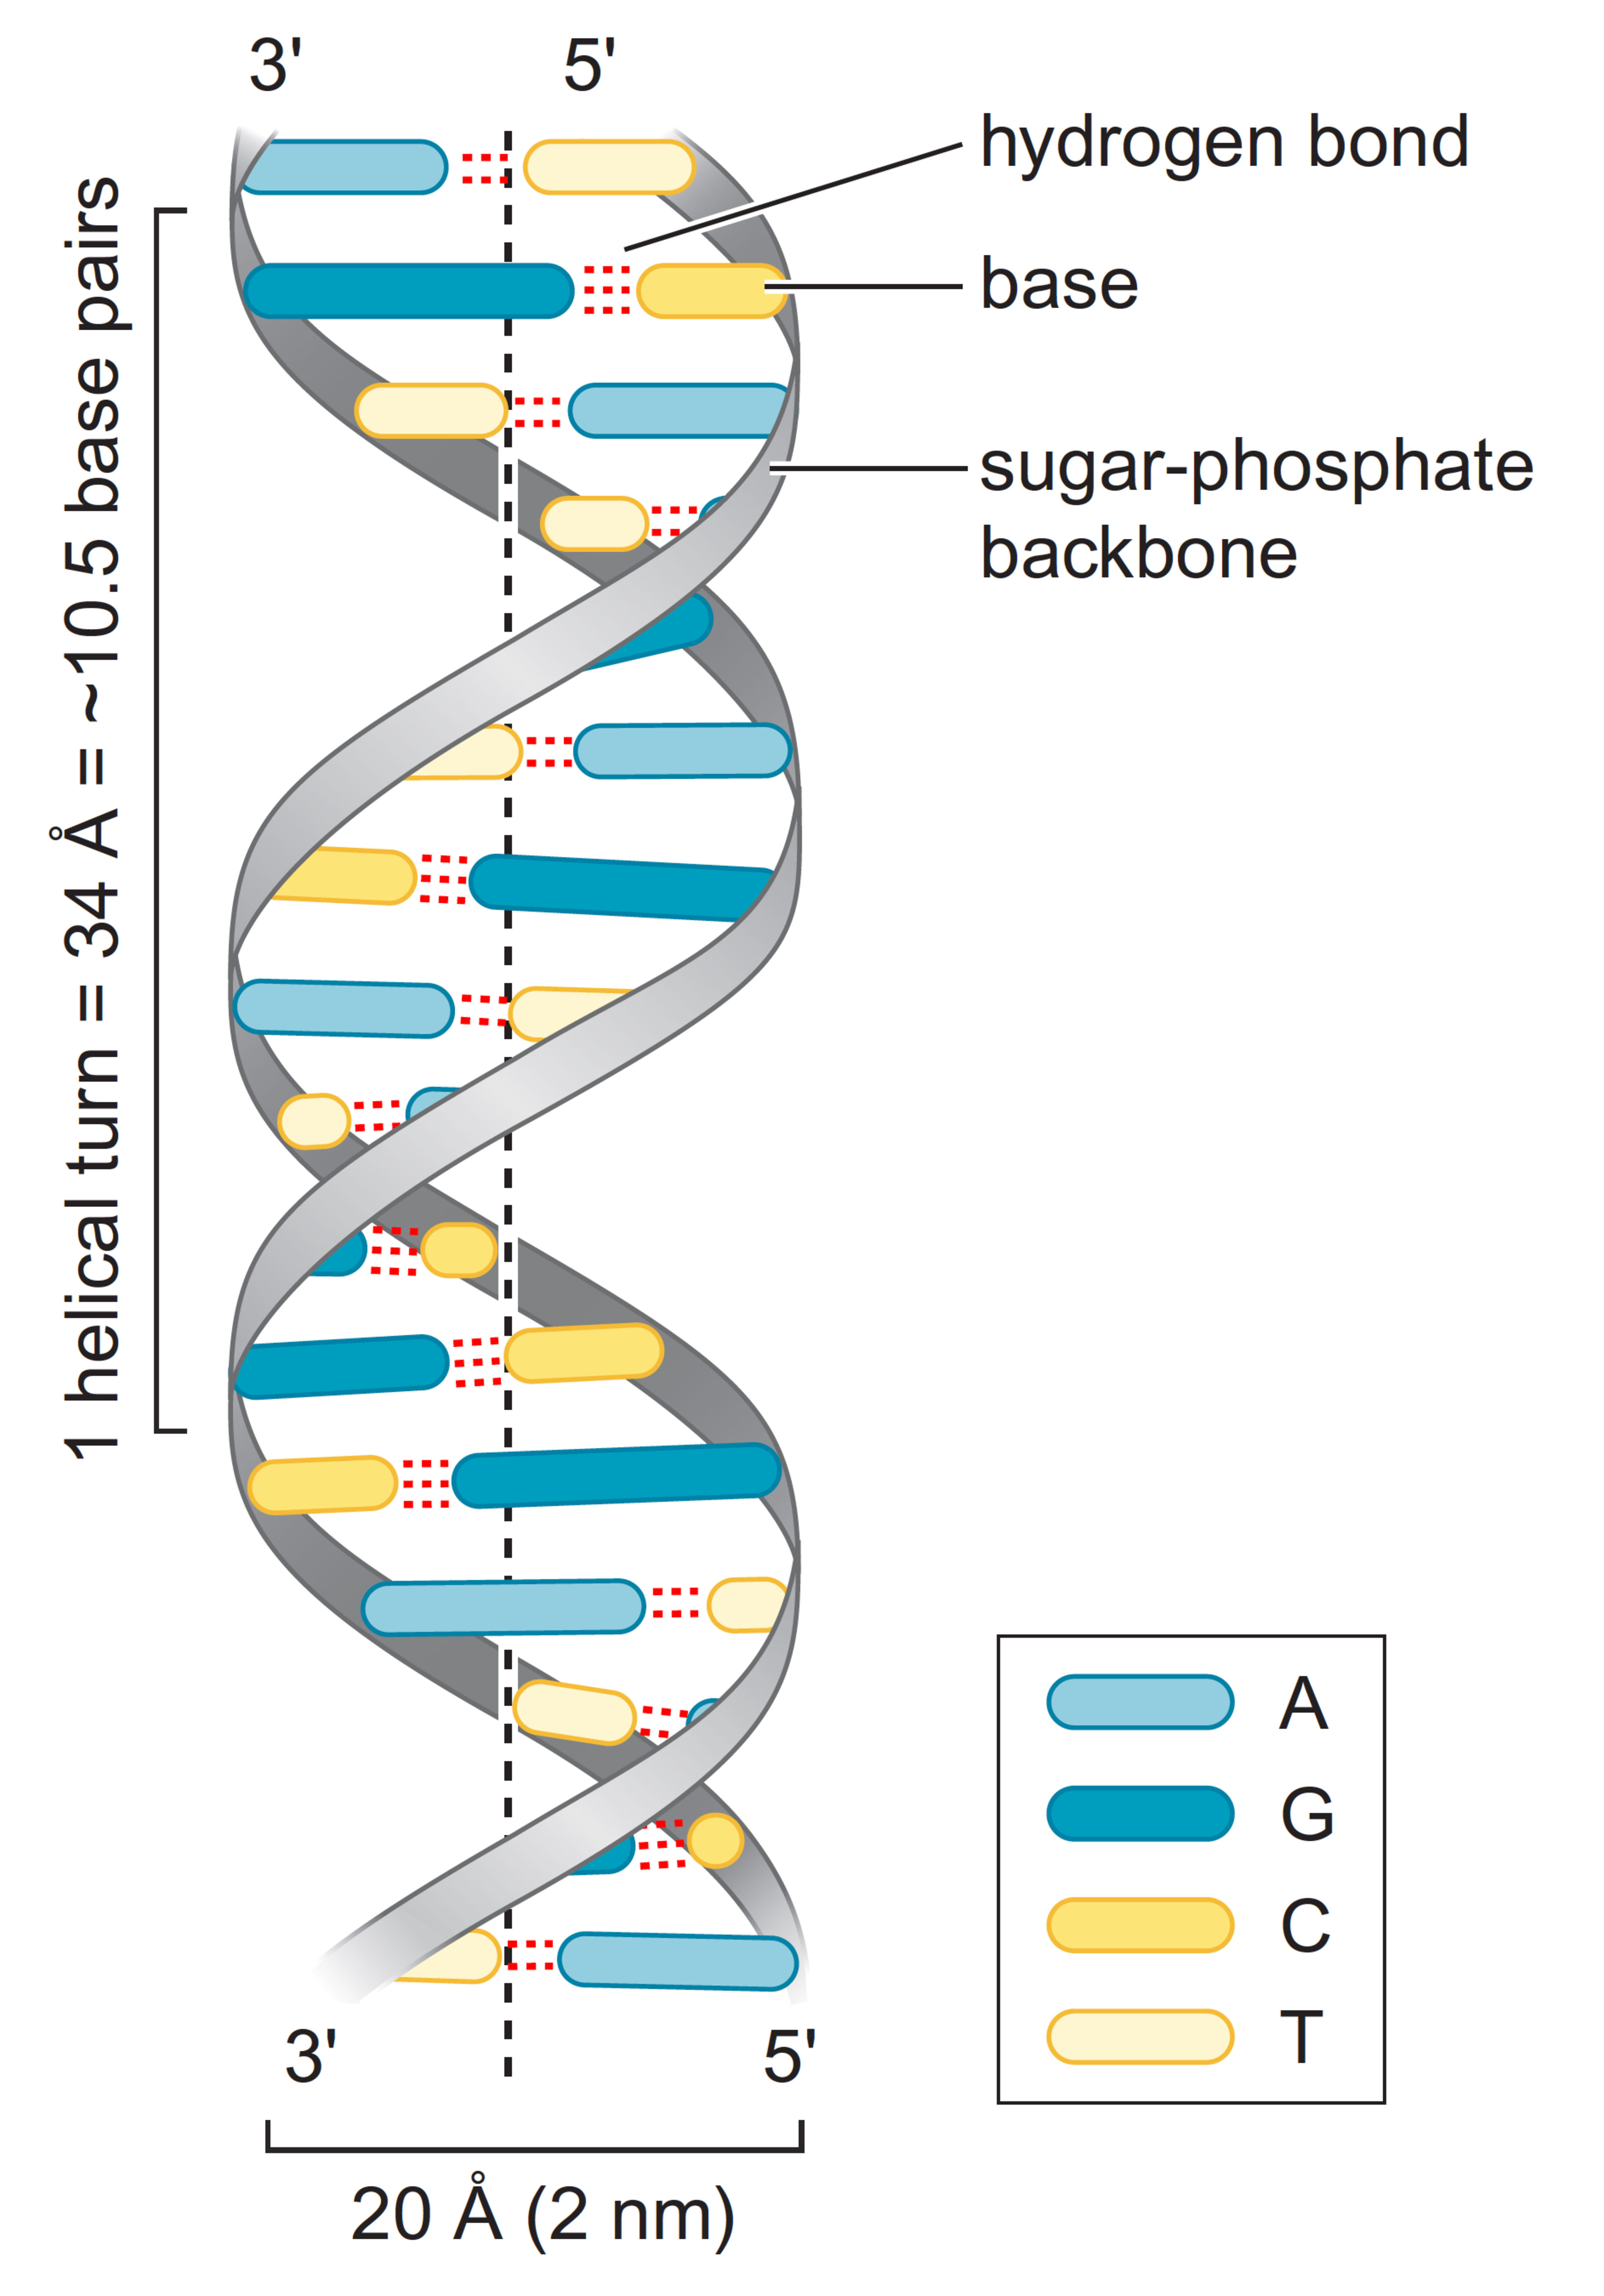
\includegraphics[width=0.4\textwidth]{Graphics/DNA/dna_structure.pdf}}                
\hspace{10mm}
\subfloat[]{\label{fig:dna_space_filled}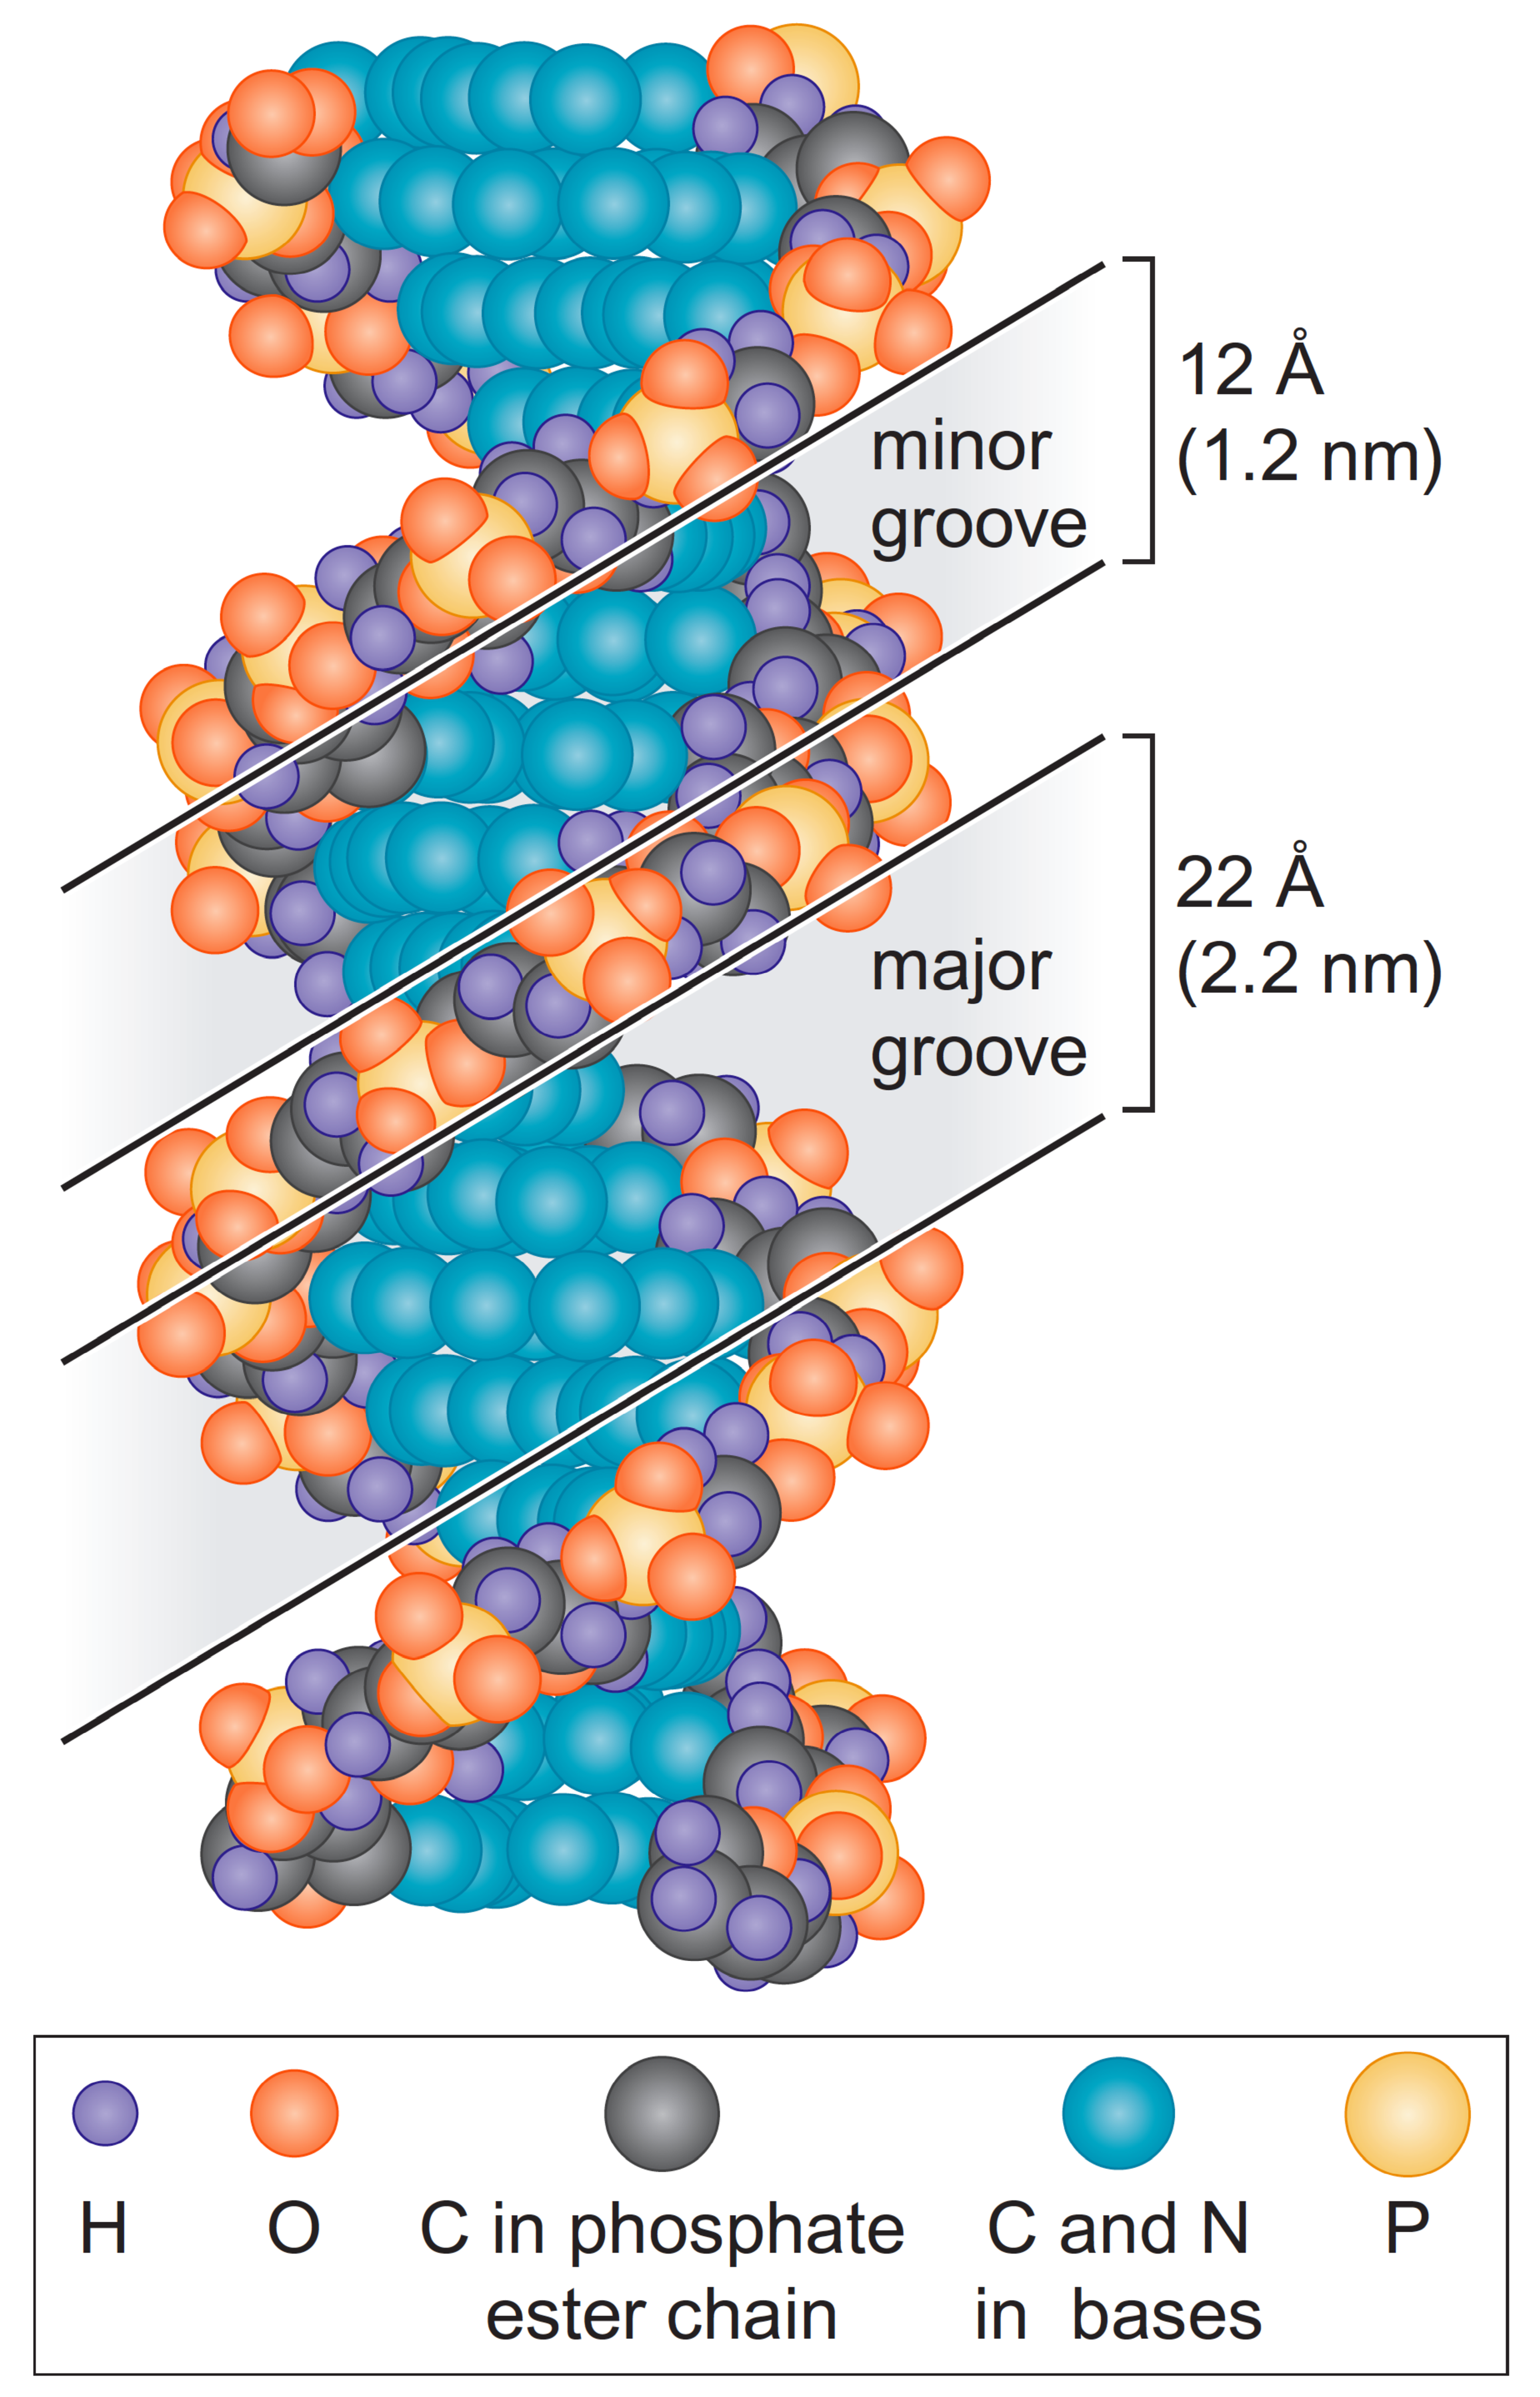
\includegraphics[width=0.4\textwidth]{Graphics/DNA/dna_space_filled.pdf}}
\caption{On the left is a schematic model of the double helix illustrating the base-pairs, and the sugar-phosphate backbone. The space-filled illustration on the right highlights the overall twist of the DNA structure with the bases located on the inside of the cylindrical structure. These illustrations are from figure 6-1 in reference \cite{Watson2003}.} 
\label{fig:dna_structure_filled}
\end{figure}
%
The first type of bases which contain two heterocyclic rings are classified as purines, called adenine (A) and guanine (G) (\figref{dna_purine}); the second type contain only a single heterocyclic ring and are classified as pyrimidines, called thymine (T) and cytosine (C) (\figref{dna_pyrimidine}). These bases participate in hydrogen bonding where two bases are connected by hydrogen bonds to form complimentary AT, and GC base-pairs. Both base-pairs have the same dimensions giving them the same planar geometry allowing the base-pairs to stack on top of each other without disturbing the sugar-phosphate backbones. The AT base-pairs are linked by two hydrogen bonds whereas the GC base-pairs are linked by three hydrogen bonds. Although individual hydrogen bonds are relatively weak when compared to covalent bonds, the bonding between the polynucleotides lies perpendicular to the fibre axis making the strength of the hydrogen bonds additive \cite{Berg2010,Watson2003}.
%
\begin{figure}[t]
\centering
\subfloat[]{\label{fig:dna_purine}\centering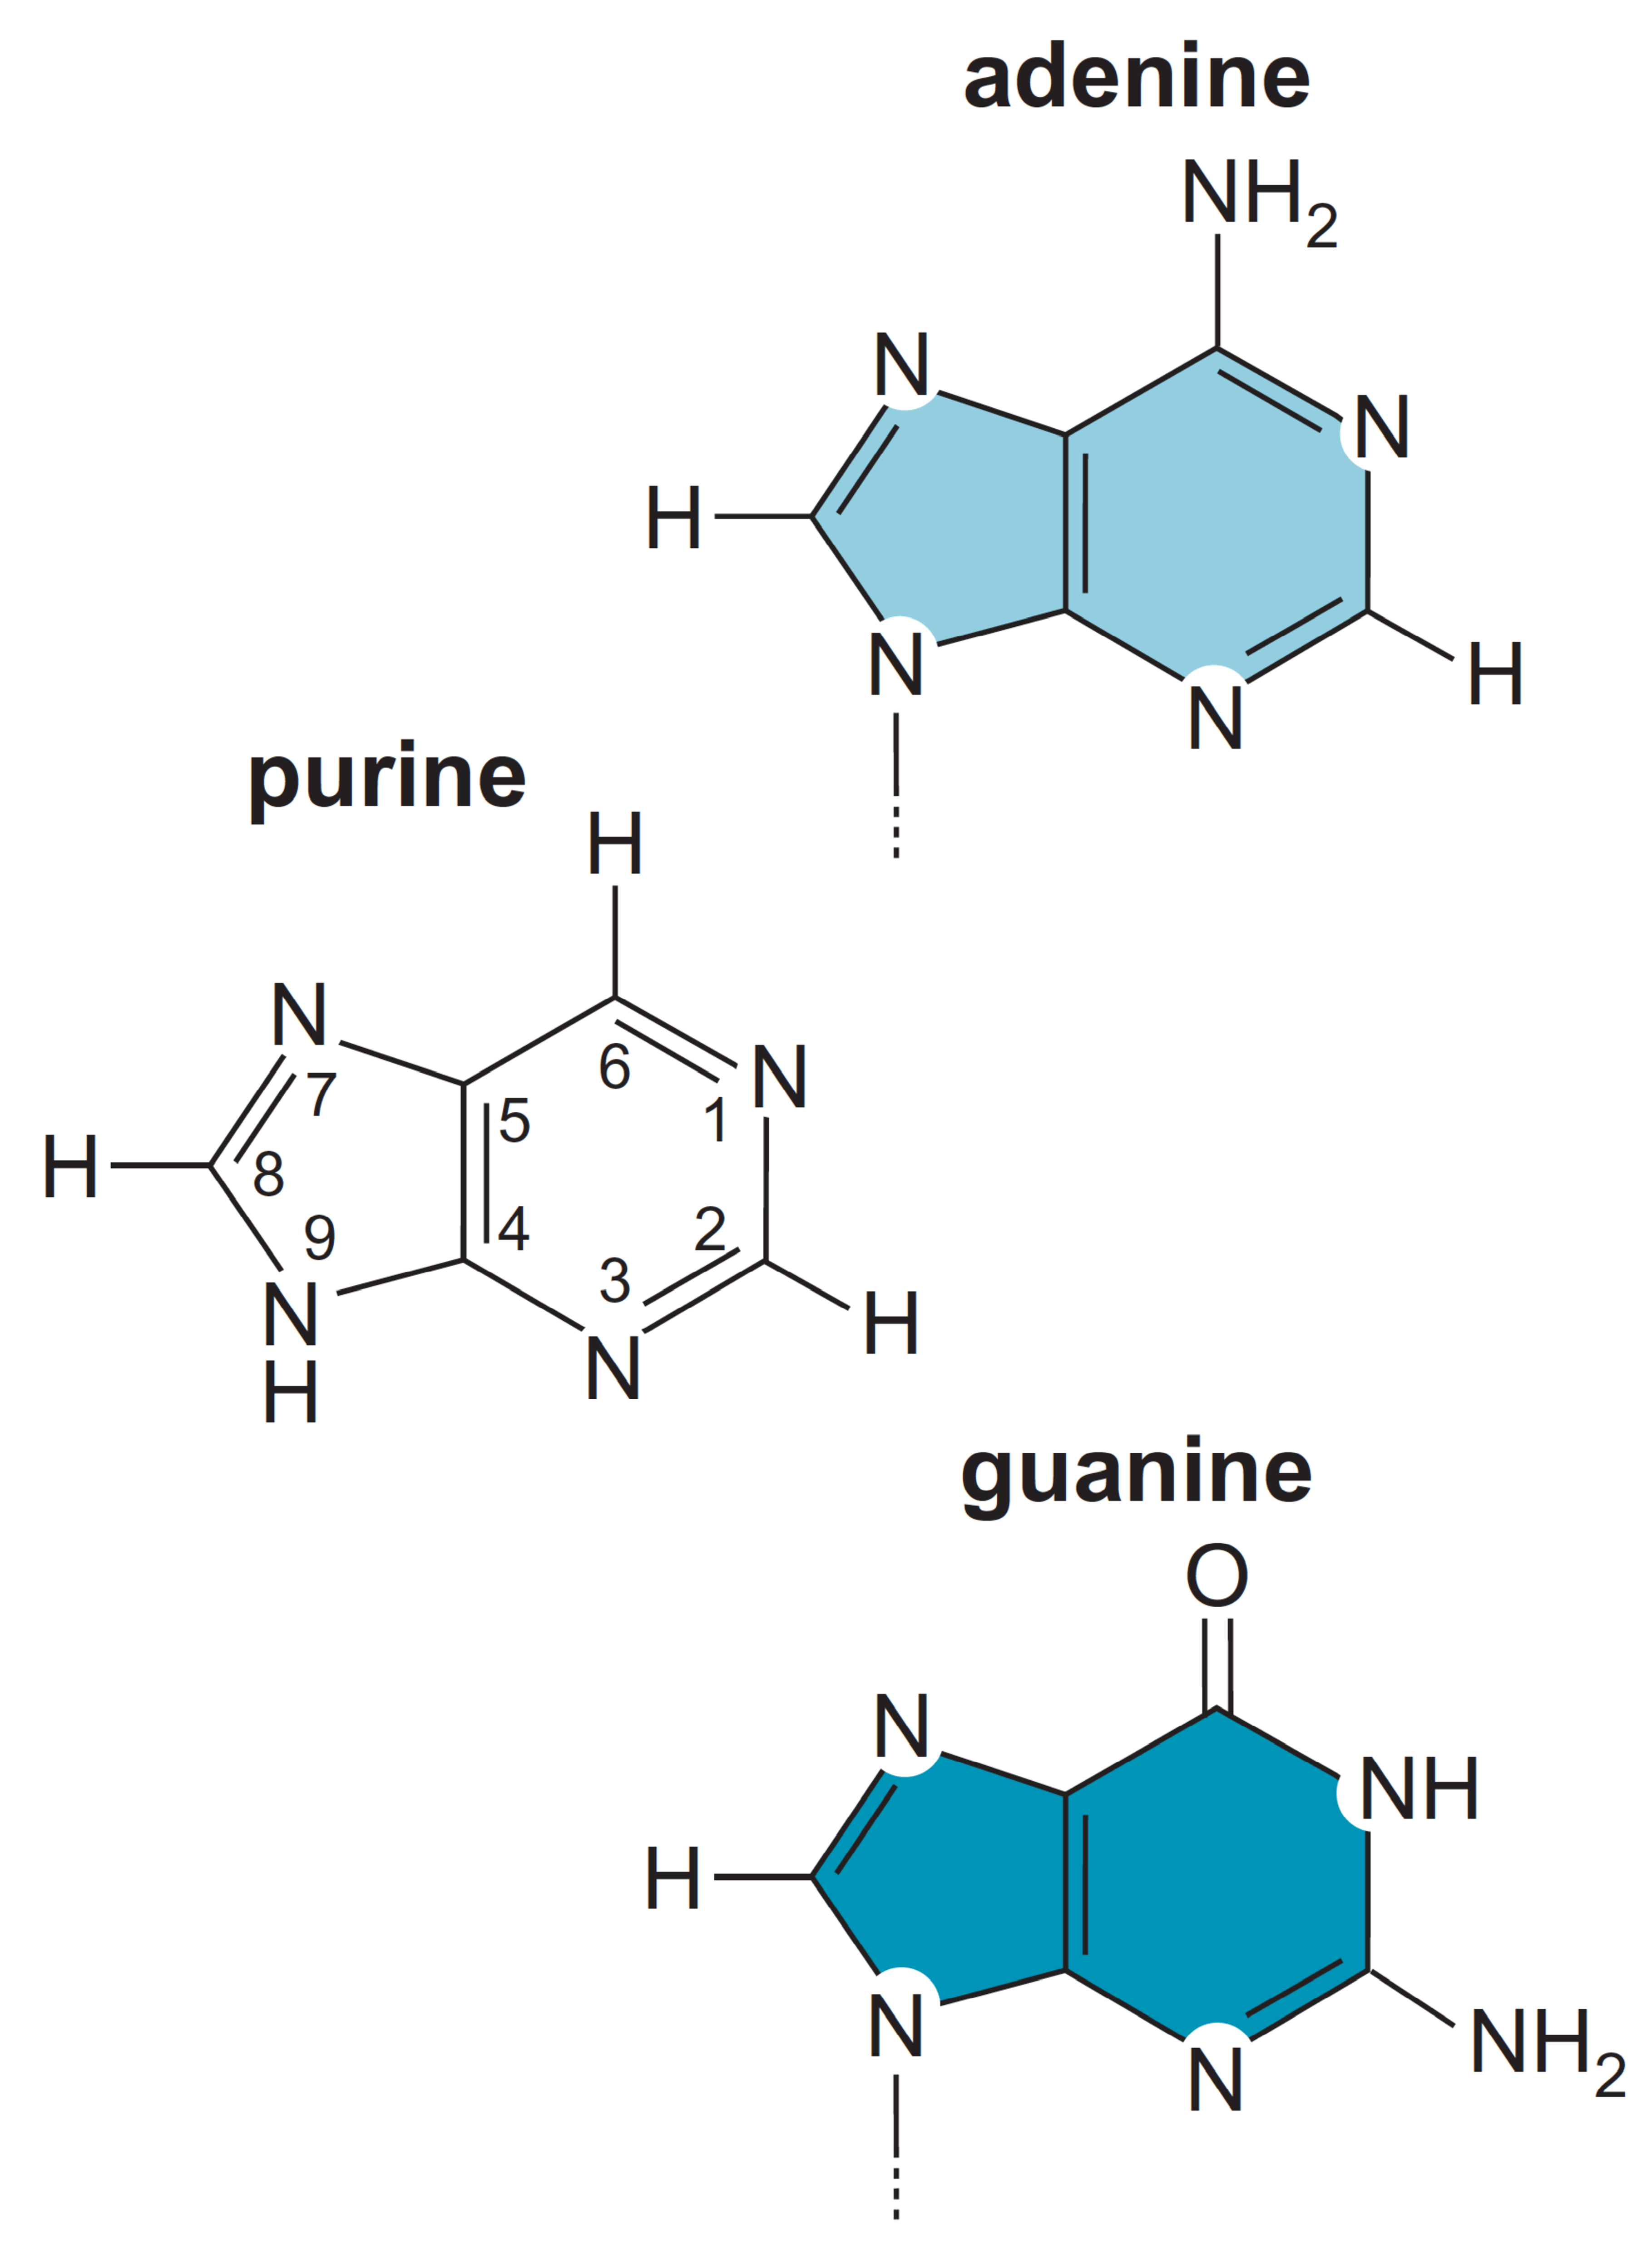
\includegraphics[width=0.3\textwidth]{Graphics/DNA/dna_purine.pdf}}
\hspace{20mm}         
\subfloat[]{\label{fig:dna_pyrimidine}\centering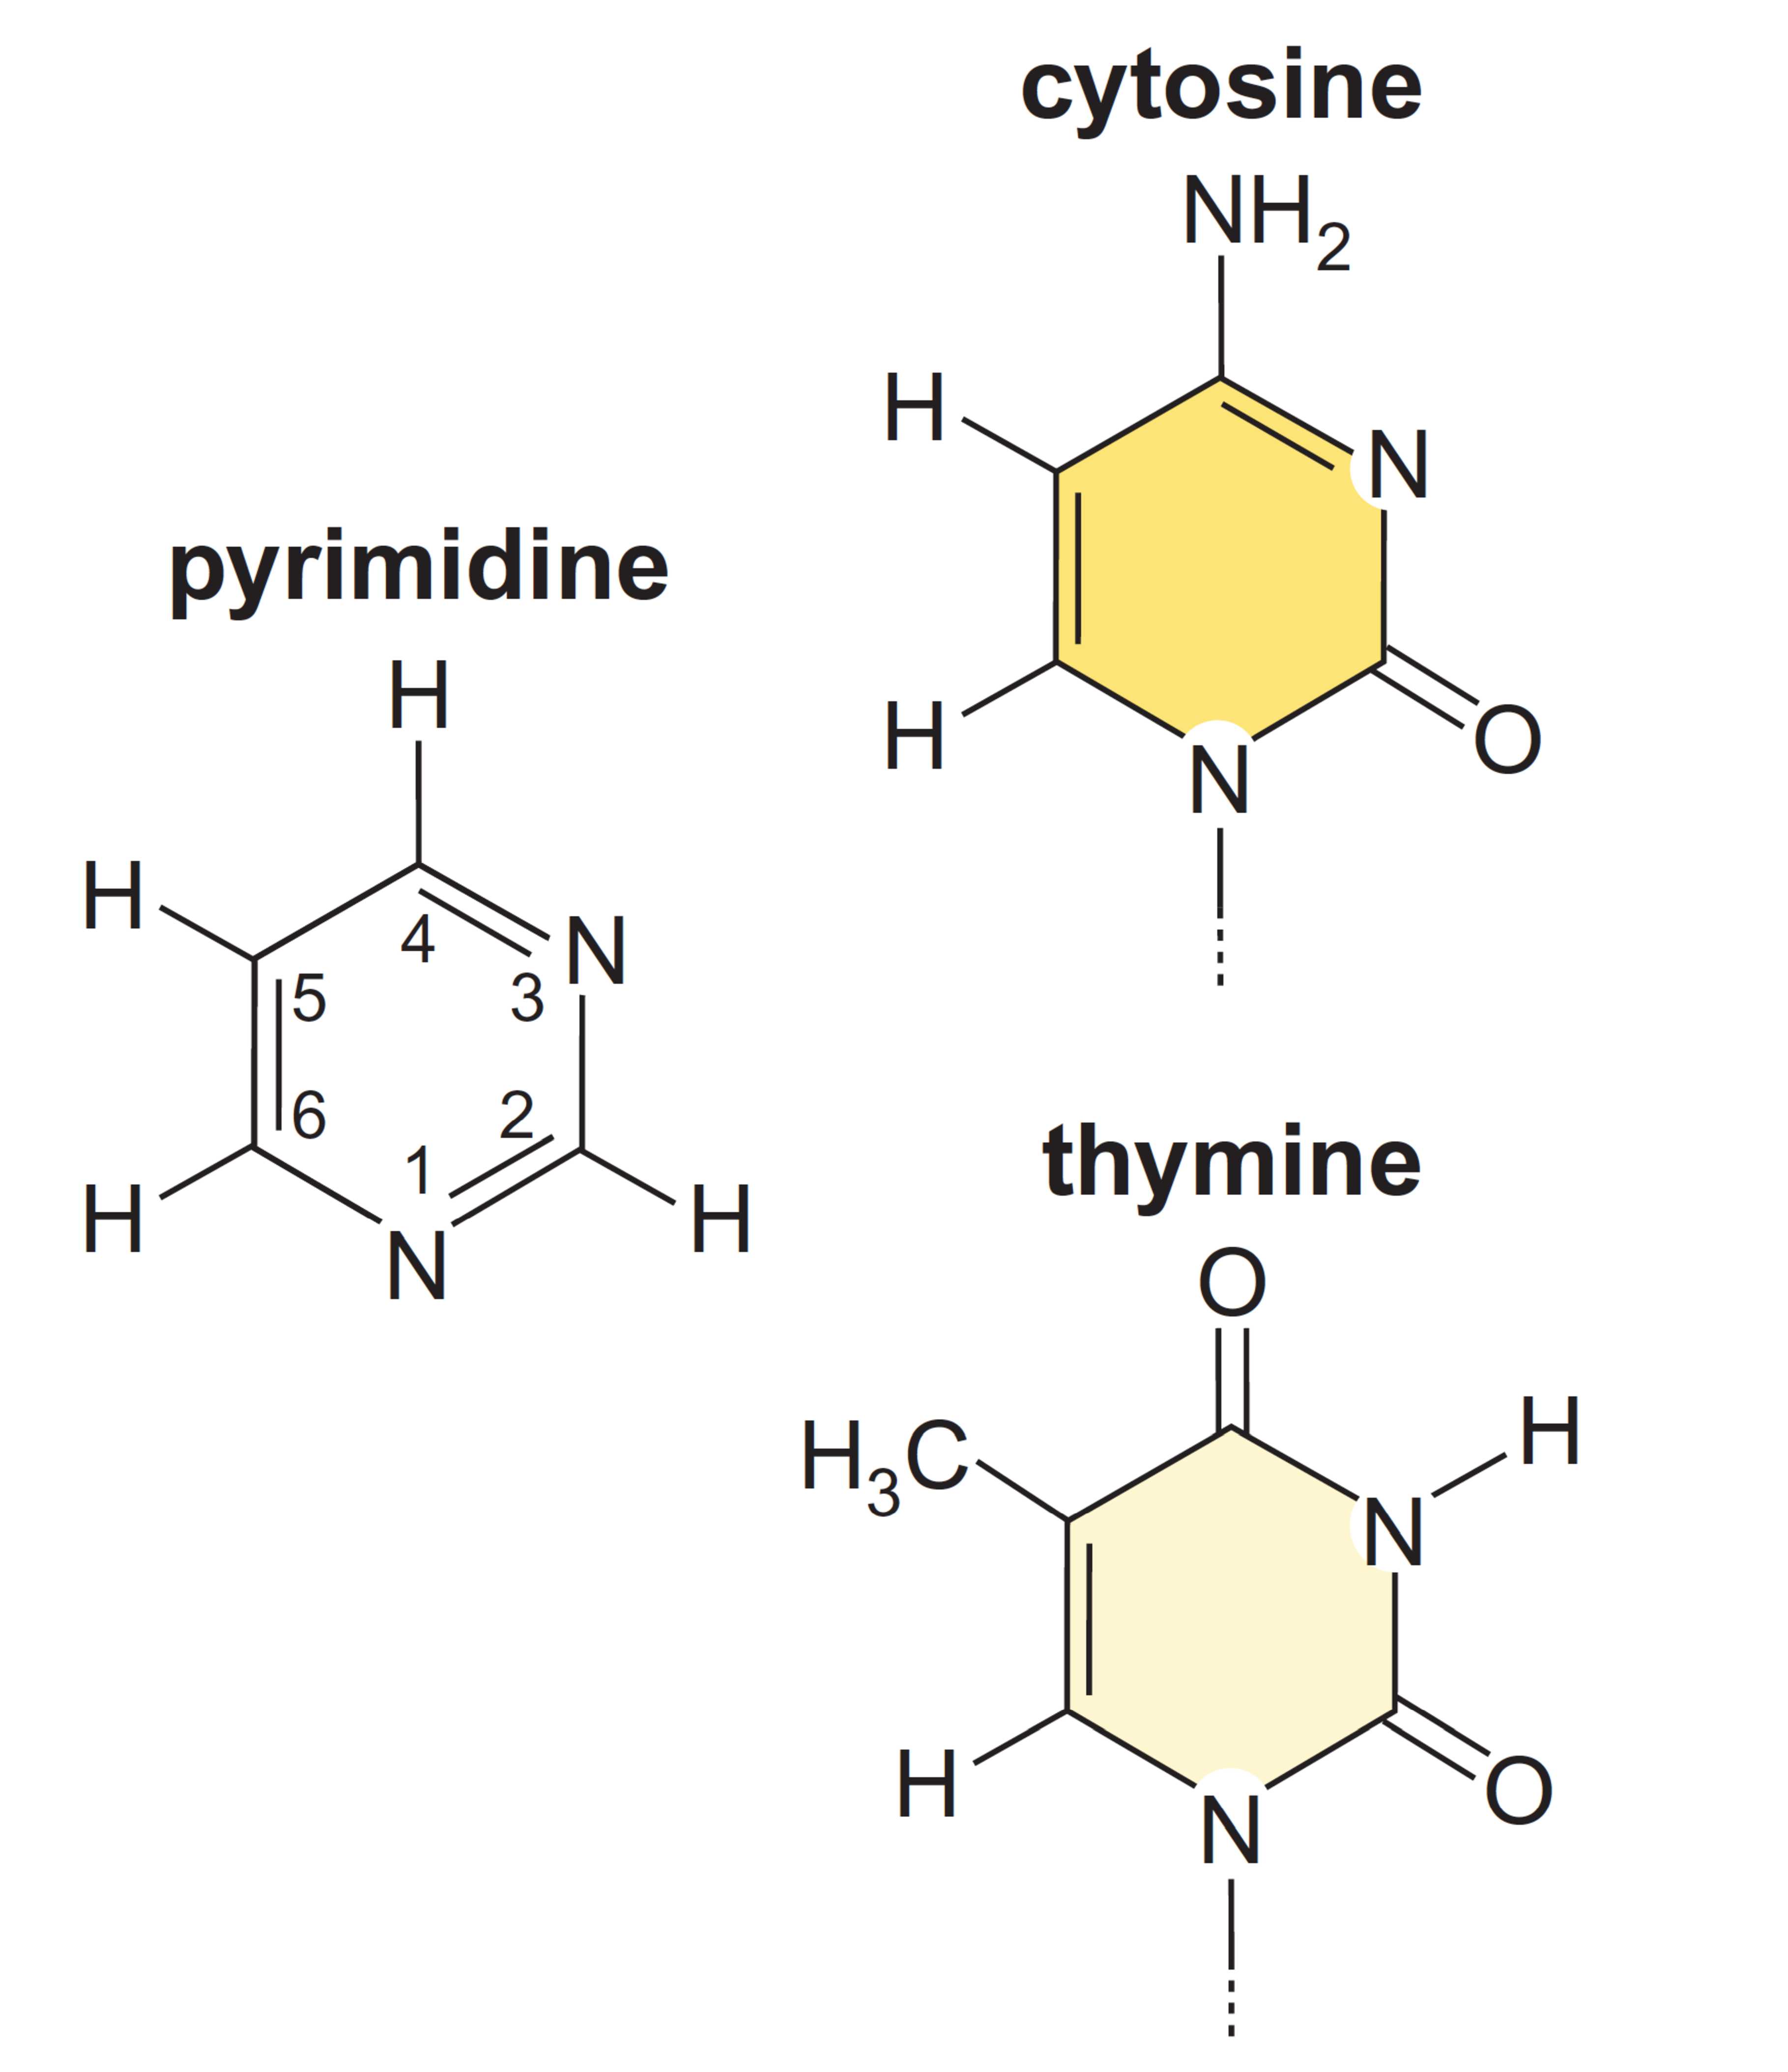
\includegraphics[width=0.3\textwidth]{Graphics/DNA/dna_pyrimidine.pdf}}
\caption{The types of bases that exist in DNA. On the left are the two purine bases that contain two heterocyclic rings, and on the right are the two pyrimidine bases that contain a single heterocyclic ring. These illustrations are from figure 6-1 in reference \cite{Watson2003}.} 
\label{fig:dna_bases}
\end{figure}
%
Although these hydrogen bonds may contribute to some of the stability of the double helix structure the main contribution comes from the stacking interaction between the bases. A combination of dipole-dipole interactions, $\pi$-$\pi$ stacking interaction, van der Waals forces and hydrophobic forces, produce an overall complex attractive interaction between the heterocyclic rings of the base-pairs. In its natural conditions, DNA is a right-handed double-helix which contains about 10.5 base-pairs per helical turn. It has two neighbouring base-pairs that are separated axially by 0.34 nm and the pitch length, the length of a helical turn of the double-helix along the central axis, is about 3.4 nm \figref{dna_structure} \cite{Watson1953}.
%
\begin{figure}[htp]
\centering
\subfloat[]{\label{fig:dna_AT_base_pair}\centering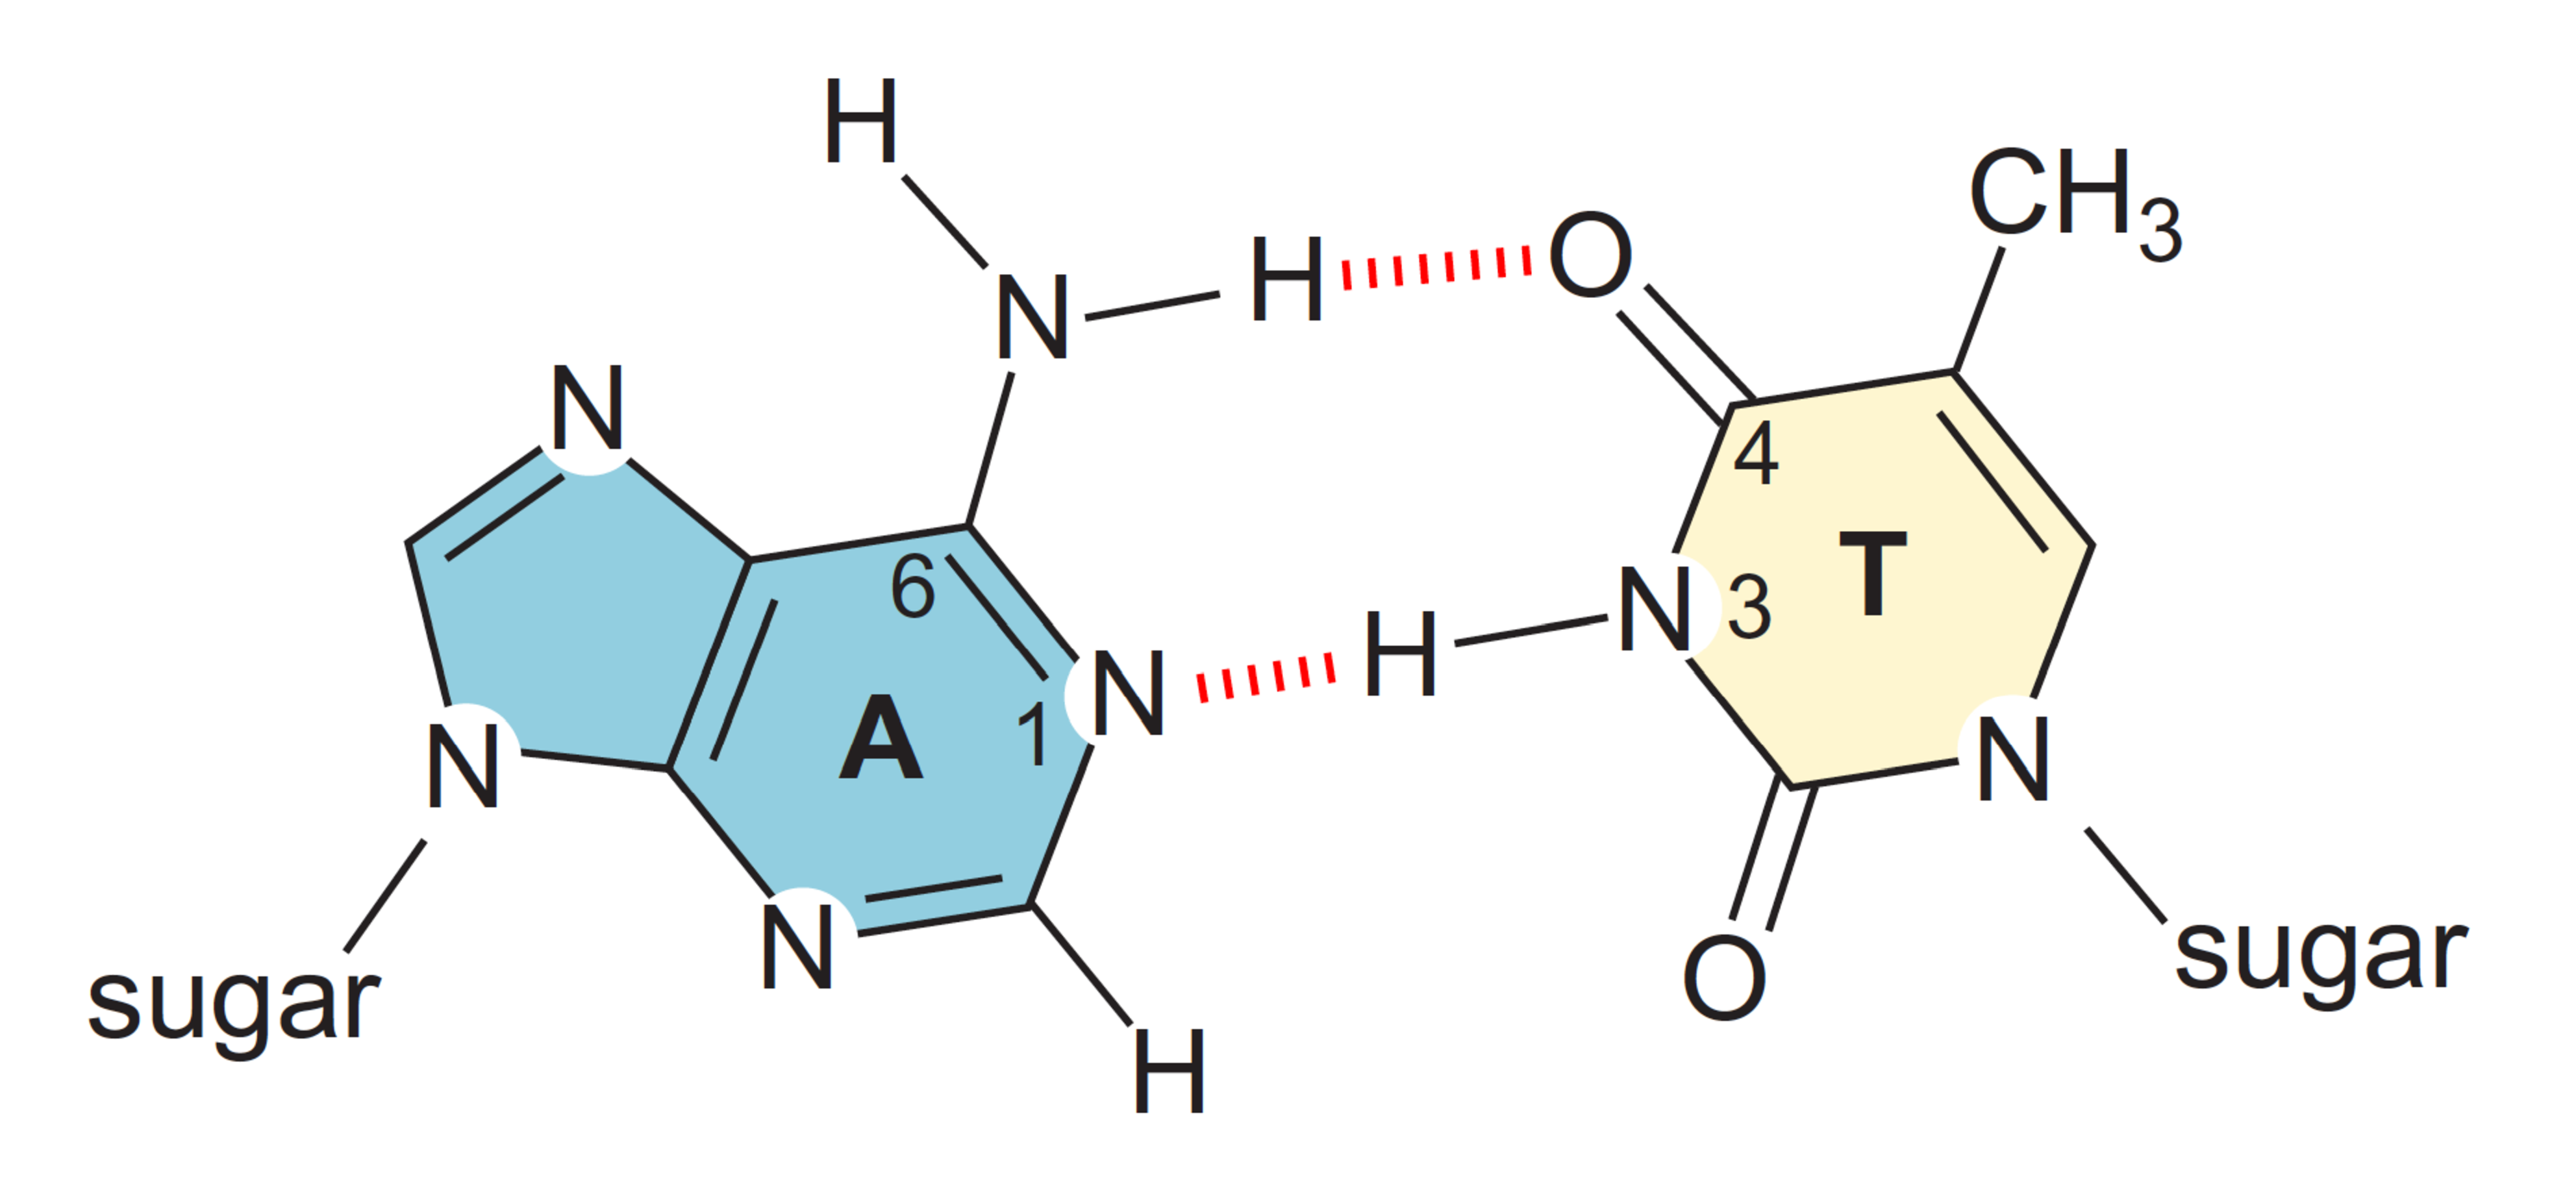
\includegraphics[width=0.4\textwidth]{Graphics/DNA/dna_base_pair_AT.pdf}}
\hspace{10mm}                
\subfloat[]{\label{fig:dna_GC_base_pair}\centering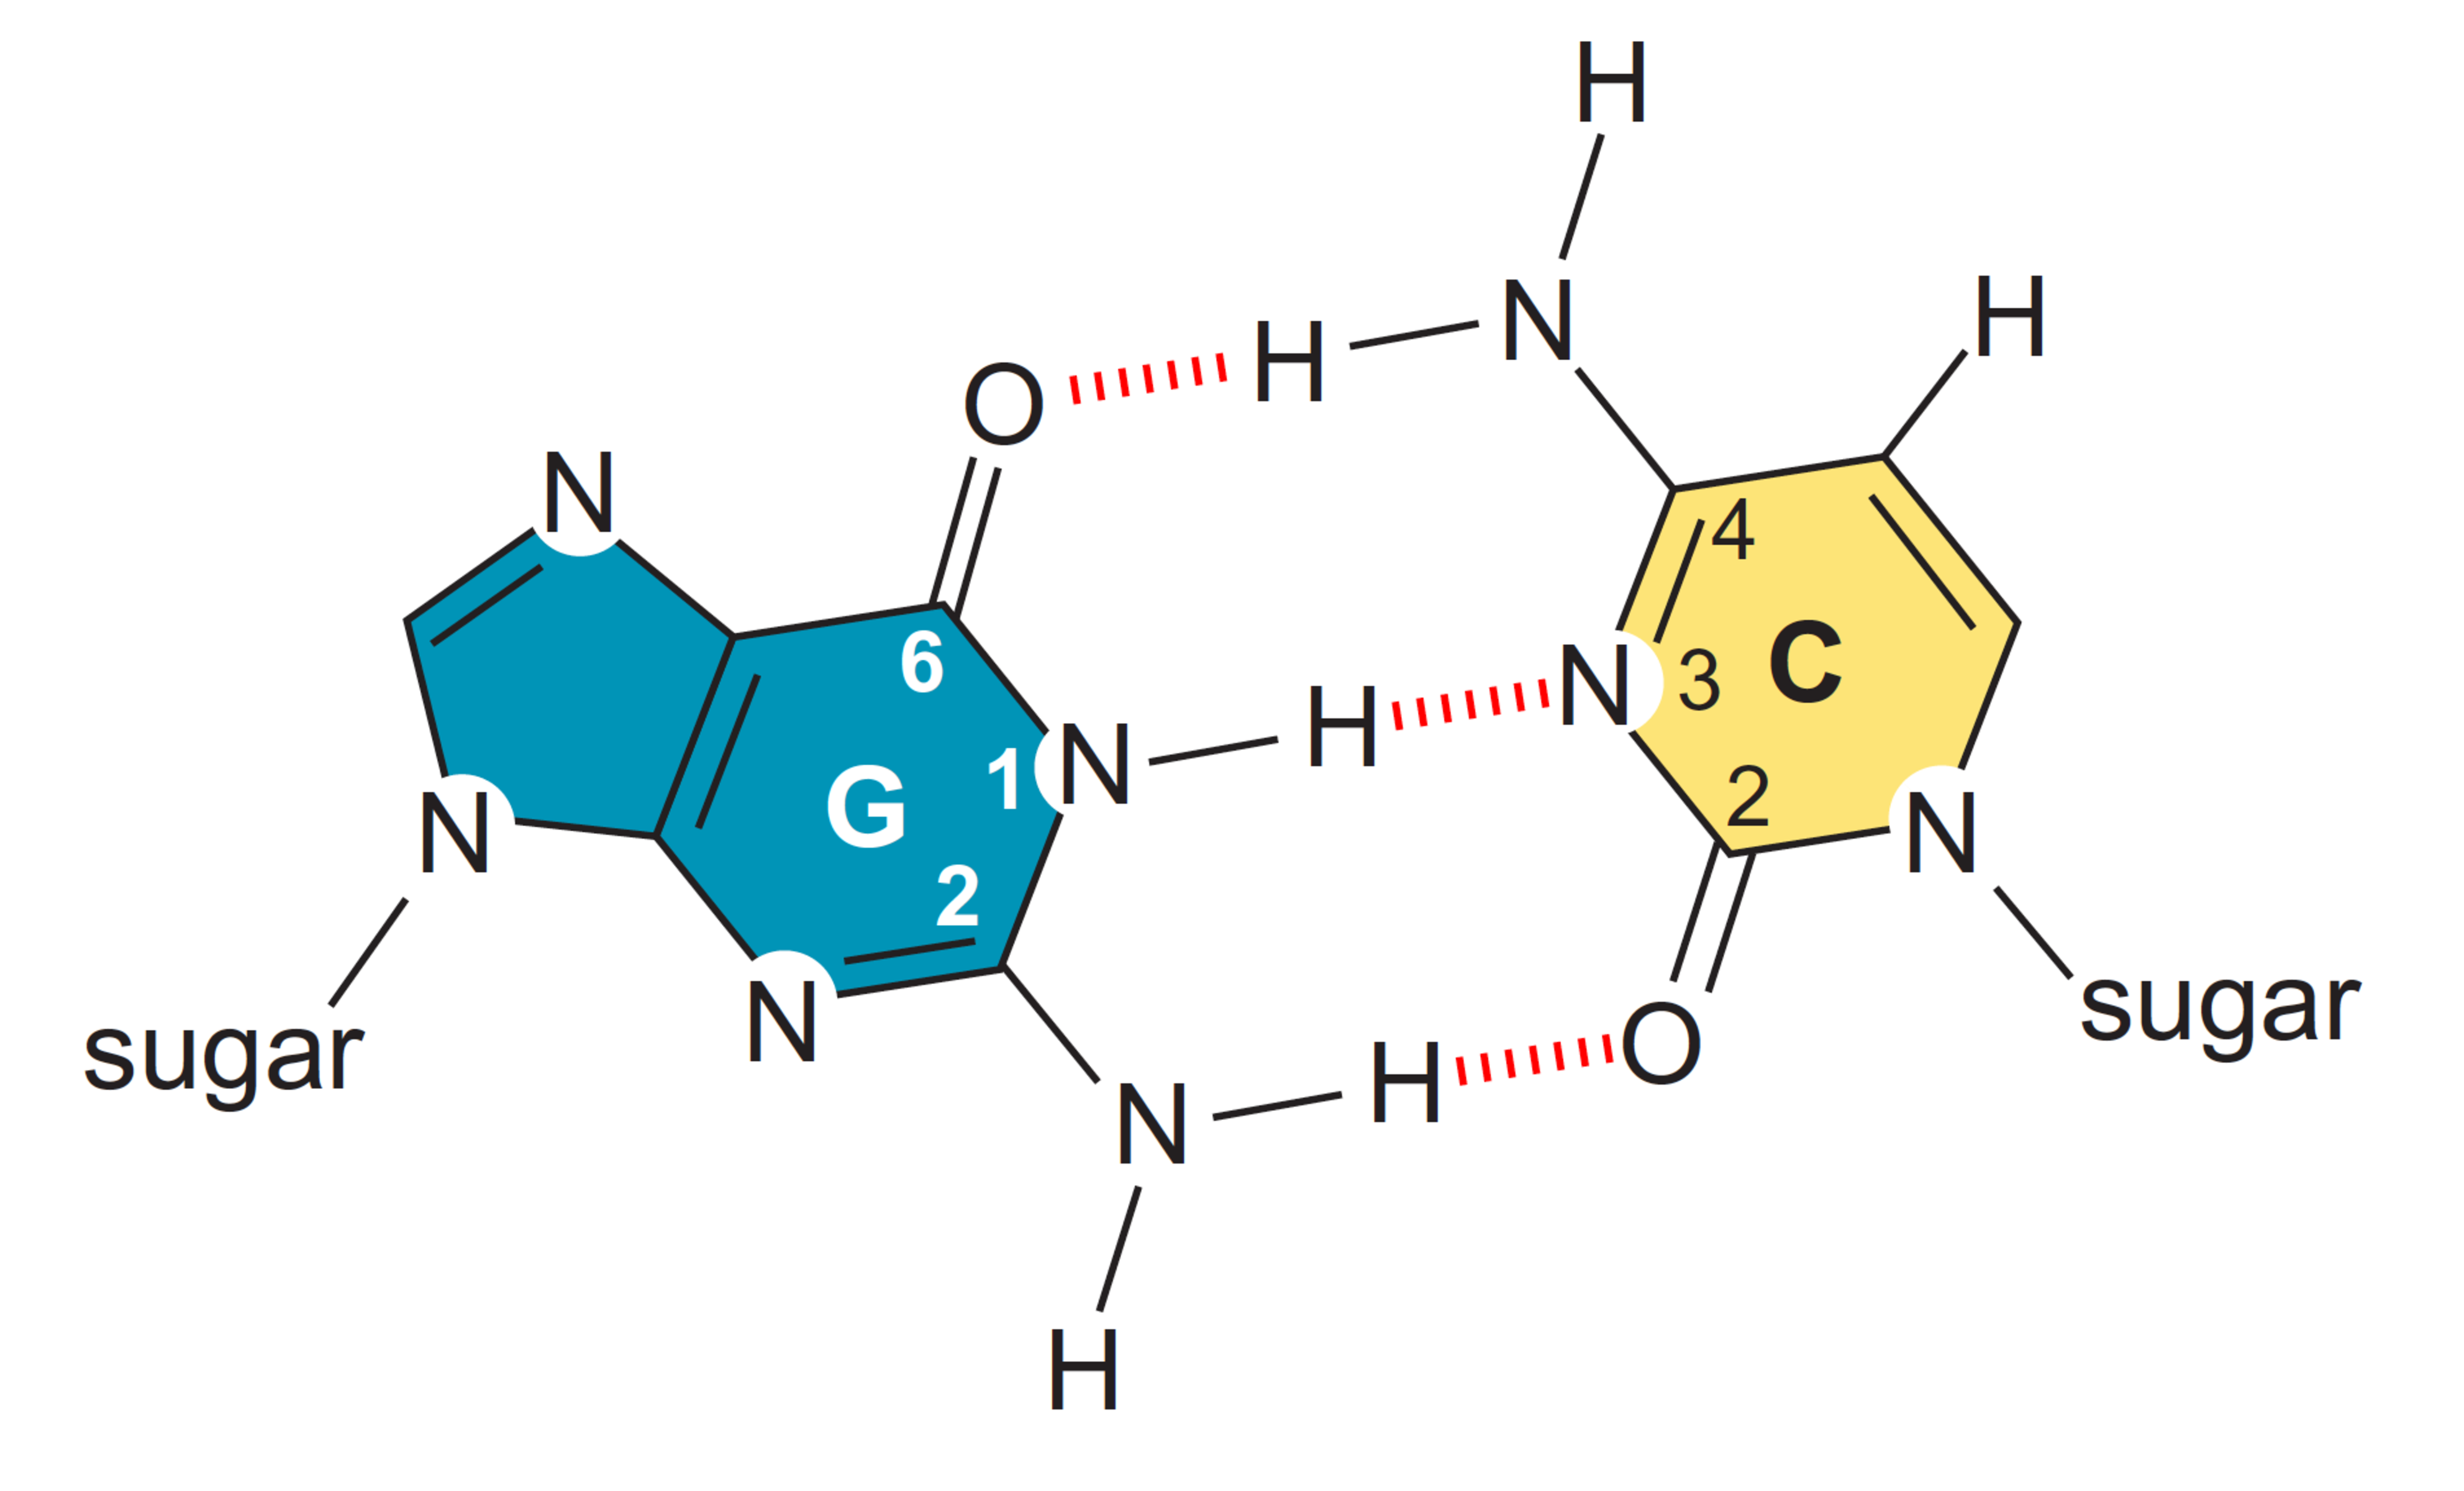
\includegraphics[width=0.4\textwidth]{Graphics/DNA/dna_base_pair_GC.pdf}}
\caption{Chemical structure of the complementary base-pairs in DNA. On the left is the adenine-thymine(AT) base-pair with two hydrogen bonds and on the right is the guanine-cytosine base-pair with three hydrogen bonds. These illiustrations are from figure 6-3 figure 6-6 in reference \cite{Watson2003}.} 
\label{fig:dna_base_pairs}
\end{figure}
%
\begin{figure}[htp]
\centering \includegraphics[scale=0.1]{Graphics/DNA/dna_schematic.pdf}
\caption{Another schematic diagram of the DNA molecule showing the different molecular groups within the backbone and base-pairs. This illustration is from figure 6-3 in reference \cite{Watson2003}.}
\label{fig:dna_schematic}
\end{figure}
%
\subsection{DNA Mechanics}

Double stranded DNA behaves like any other polymer in aqueous solution, exchanging energy with its surrounding environment at thermal equilibrium. The thermal agitation causes the DNA to bend and curve locally by small forces that continuously change the macroscopic configuration of the molecule. Commonly described as Brownian motion this has the effect of reducing the end-to-end distance of the molecule, maximising its conformational entropy such that its most probable configuration is a random coil. Purely entropic in origin, the free energies of deformations of the molecule are of order $kT \sim 4$ pN nm which sets the lower limit of the forces needed to stretch a DNA molecule to its contour length \cite{Harris2004,Strick2003}. 

Some of the first experiments measuring the entropic elasticity of DNA were conducted by Smith et al (1992). Using a method where they chemically attached one end of the DNA to a glass surface and tethered the other end to a magnetic bead they were able to measure the force extension of DNA using a combination of magnetic fields and hydrodynamic drag \cite{Smith1992}. The results shown from their experiments in \figref{fig1_Bustamante2000} describe DNA having a linear relationship in the limit of low forces with a Hooke's constant that is inversely proportional to the length of the molecule. Here we see the FJC model agreeing well with such force extension curves for DNA. As the applied force increases the experimental results clearly dismiss the FJC model as a suitable candidate for describing DNA.

A better description is provided by the Worm Like Chain (WLC) model which considers DNA to be a continuous flexible worm-like chain \cite{Marko1995}. In this model the persistence length $L_{p}$ is a quantitative measure of chain stiffness which defines a length scale over which segments of the counter length are correlated. Since the FJC model is only flexible between fixed segments and ignores the bending fluctuations of the segments themselves, the WLC provides a more realistic description of entropy change in stiffer polymers. 
%
\begin{figure}[h]
\centering
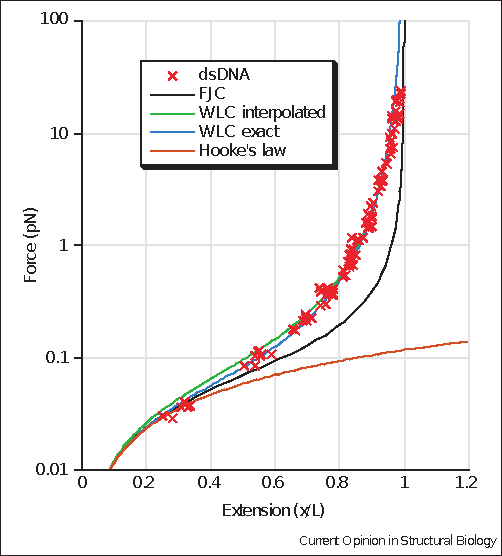
\includegraphics[scale=1]{Graphics/DNA/fig1_Bustamante2000.pdf}
\caption{Force extension behaviour of double stranded DNA. The experimental data taken from Smith et al. (1992) is fitted to the WLC model using the modified WLC interpolated formula \eqref{wlc_num_approx}, the exact WLC model solved numerically, and the linear spring \eqref{wlc_num_approx_small} are also shown. In these plots $L_{p}=53$ nm where the FJC assumes twice the persistence length. This original plot was reported in \cite{Bustamante2000}.}
\label{fig:fig1_Bustamante2000}
\end{figure}
%
The first complete treatment of the WLC model was achieved by Marko and Siggia using two different methods; for the exact solution they numerically evaluated a line integral of two terms in the WLC model where the first term described the resistance of the chain bending, and the second term described the stretching energy resulting from an applied force. Following the terminology used in \cite{Marko1995} we describe the DNA conformations by a space curve $\mathbf{r}(s)$ of a contour length, $L$, where $s$ is the arc length, and the energy in the WLC model is expressed as:
%
\begin{equation}
E_{wlc}=k_{B}T \int_{0}^{L}ds \left(  \frac{A}{2}\left|\frac{d\mathbf{r}\left(s\right)}{ds}\right|^{2} -F\cos\left(\theta\left(s\right)\right)\right)
\end{equation}
%
where $\theta\left(s\right)$ is the angle between $\mathbf{r}(s)$ and the axis along the direction of force $F$.  In the second method they expanded the first term to the quadratic order that led to the Gaussian approximation of the line integral. They were able to derive an interpolation formula that was close to the exact numerical solution of the force-extensions  \cite{Marko1995,Bustamante1994}:
%
\begin{equation}
\label{wlc_num_approx}
F\left(x\right)=\left(\frac{k_{B}T}{L_{p}}\right)\left[\frac{1}{4\left(1-\frac{x}{L}\right)^{2}}-\frac{1}{4}+\frac{x}{L}\right]
\end{equation}
%
where $L$ is the length of the molecule, $L_{p}$ is the persistence length and $x$ is the extension. For small values of $\frac{x}{L}$, the approximation simplifies to
%
\begin{equation}
\label{wlc_num_approx_small}
F\left(x\right)=\frac{3 k_{B}T}{2L_{p}}\left(\frac{x}{L}\right)
\end{equation}
%
which demonstrates that the molecule behaves as a linear spring with a stiffness constant $k_{DNA}=\frac{3 k_{B}T}{2LL_{p}}$. Further corrections, and improvements have been made to \eqref{wlc_num_approx} to include effects of stretching DNA in physiological buffer \cite{Wang1997,Bouchiat1999}. For the results shown in \figref{fig1_Bustamante2003} the stretch modulus was found to be approximately 1000 pN in a buffer solution \cite{Bustamante2000}. The failure to account for the enthalpic correction at small forces (5-10 pN) leads to underestimation of $L_{p}$ resulting in a deviation from the model above 10 pN \cite{Bouchiat1999,Wang1997}. The experimental results shown in \figref{fig1_Bustamante2000} were taken from Smith et al. (1992) where the persistence length of DNA in the WLC model was $L_{p}\sim$ 53 nm in order to fit the experimental data. Other experiments including the more recent experiment by Van Maneren et al. (2009) have reproduced these force extension curves for DNA which have shown that the predictions of the WLC model provide an excellent agreement with the data measured \cite{Cluzel1996,Wang1997,Smith1996,VanMameren2009}. This can also be observed in \figref{fig1_Bustamante2000}. 
%
\begin{figure}[htp]
\centering
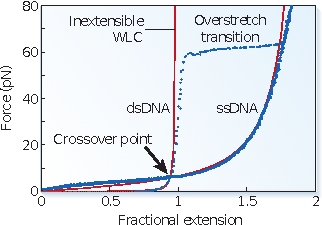
\includegraphics[scale=1.5]{Graphics/DNA/fig1_Bustamante2003.pdf}
\caption{Force extension behaviour of DNA and ssDNA \cite{Bustamante2003}. }
\label{fig:fig1_Bustamante2003}
\end{figure}
%
At forces above 65 pN DNA structurally changes under mechanical stress causing the DNA molecule to extend 1.7 times the original length. We see this extra length being released over a narrow range of force shown by the plateau in \figref{fig1_Bustamante2003}. Experiments have highlighted that the force at which the over-stretching transition occurs is dependent on the details of terminal attachments, $\sim 65$ pN if the molecule is torsionally relaxed at both ends, and $\sim 110$ pN if it is not. Two competing models \cite{VanMameren2009} have been proposed to describe the structural behaviour in this overstretched region: In the first model it is thought that DNA gradually unwinds under tension, with the base-pairs intact, into the S-form DNA resembling a parallel ladder.  The second model interprets the overstretched phase as a denatured DNA resulting from strand separation caused by breaking of hydrogen bonds between complementary bases. Recent experiments show that there is a region where both these models can coexist with base-pair melting causing strand separation from DNA to single stranded DNA (ssDNA) \cite{VanMameren2009,Williams2009,Fu2010}. 

\subsection{DNA Models}

In an attempt to study the DNA transcription process Peyrard et al. \cite{Peyrard1989a} found that developing a mathematical model that included the roles played by the RNA polymerase enzymes would be far too complex a task. Similarities were noted with DNA thermal denaturation, a mechanism where the backbone DNA strands separate by heating, also known as DNA melting. This function initiates locally by the formation of bubbles within the DNA structure and therefore was considered to be a preliminary step in understanding the transcription process \cite{Peyrard1989a, Dauxois1993a, Dauxois1993, Peyrard2004}. 

Simplifying the DNA structure to a 1D ladder system Peyrard et al. were able to write a  Hamiltonian as a function of base pair separation that included temperature independent parameters, and then studied the statistical mechanics of the system by employing the transfer integral method. The model has two degrees of freedom where in each strand the displacements of the $n^{th}$ base from their equilibrium position is labelled $u_{n}$ and $v_{n}$ along the direction of the hydrogen bond that connects base pair. The structure is considered homogeneous and periodic with each nucleotide base being represented by a point mass $m$ \cite{Peyrard1989a}.

The effective base pair potential $V$ was modelled by a Morse potential to represent the 2 or 3 hydrogen bonds that connect the two bases in a pair, and along each backbone  strand the neighbouring bases are connected by a stacking harmonic potential that has a stiffness constant $\kappa$. For system with $N$ base pairs, the Hamiltonian is expressed as \cite{Peyrard1989a},
%
\begin{equation}
H=\sum_{n}\frac{m}{2}\left( \dot{u}_{n}^{2} + \dot{v}_{n}^{2}  \right) +\frac{\kappa}{2}\left(u_{n}-u_{n-1}\right)^{2} + \frac{\kappa}{2}\left(v_{n}-v_{n-1}\right)^{2}+V \left(u_{n}-v_{n}\right)
\label{pb_model_hamiltonian}
\end{equation}
%
with
%
\begin{equation}
V \left(u_{n}-v_{n}\right) = D\left[\exp \left(-a\left( u_{n}-v_{n} \right) \right) -1\right]^{2}
\label{pb_model_bp_potential}
\end{equation}
%
where $D$ is the dissociation energy of the base pair, and $a$ is the parameter that sets the spatial range of the base pair potential. The first term in \eqref{pb_model_hamiltonian} represents the kinetic energy of the system, the second term corresponds to the effect of stretching along the backbone, and the third term represents the interaction of the base pair. 

Further simplifications are made to the Hamiltonian by transforming the co-ordinate system into variables that represent the in-phase $x_{n}$, and out-of-phase $y_{n}$ motions of the base positions. The transformations are \cite{Peyrard1989a}
%
\begin{equation}
x_{n}=\frac{u_{n}+v_{n}}{\sqrt{2}}
\end{equation}
%
\begin{equation}
y_{n}=\frac{u_{n}-v_{n}}{\sqrt{2}}
\end{equation}
%
which readily separates the Hamiltonian to give 
%
\begin{equation}
H = H\left(x_{n}\right) + H\left(y_{n}\right)
\end{equation}
%
with 
%
\begin{align}
H\left(x\right) &= \sum_{n}\frac{p_{n}^{2}}{2m}+\frac{\kappa}{2}\left(x_{n}-x_{n-1}\right)^{2} \\
H\left(y\right) &= \sum_{n}\frac{q_{n}^{2}}{2m}+\frac{\kappa}{2}\left(y_{n}-y_{n-1}\right)^{2} + V'\left(y_{n}\right)
\end{align}
%
where $p_{n}=m\dot{x}_{n}$, $q_{n}=m\dot{y}_{n}$ and $V'\left(y_{n}\right)=V\left(\sqrt{2}y_{n}\right)$. In the partition function integral we find that the momentum terms and the terms in $x_{n}$ integrate analytically to provide a constant factor in the total partition function. For the remaining terms in $y_{n}$ the partition function integral can be written as  \cite{Peyrard1989a}
%
\begin{equation}
Z\left(\beta\right)=\int \prod^{N}_{n=1} \,dy_{n}\exp\left(-\beta H\left(y_{n},y_{n-1}\right) \right)\delta\left(y_{N}-y_{1}\right)
\label{pfi1}
\end{equation}
%
with the delta function fulfilling a periodic boundary condition.  This partition function integral can also be expressed using a product of Boltzmann factors to give
%
\begin{equation}
Z\left(\beta\right)=\int \prod^{N}_{n=1} \,dy_{n}\left[ \prod_{i=1}^{N}\exp\left(-\beta f\left(y_{n},y_{n-1}\right) \right)\right]\delta\left(y_{N}-y_{1}\right)
\label{pfi2}
\end{equation}
%
where the term $f\left(y_{n},y_{n-1}\right)$ can be generalised to a sum of the backbone interactions $W\left(y_{n},y_{n-1}\right)$ and the base pair interactions $V'\left(y_{n}\right)$, that is,
%
\begin{equation}
f\left(y_{n},y_{n-1}\right)= W\left(y_{n},y_{n-1}\right) +V'\left(y_{n}\right) = \frac{\kappa}{2}\left(y_{n}-y_{n-1}\right)^{2} + V'\left(y_{n}\right)
\end{equation}
%
In this one-dimensional problem the integral can be evaluated exactly in the thermodynamic limit of a large system using the eigenvalues and eigenfunctions of a transfer matrix. Introducing the the transfer integral operator $T$ we have an eigenvalue equation \cite{Peyrard1989a}
%
\begin{equation}
\int dy' T\left(y,y'\right)\psi_{i}\left(y'\right) =\lambda_{i}\psi_{i}\left(y\right)
\end{equation}
%
with
%
\begin{equation}
T\left(y,y'\right) = \frac{\kappa}{2}\left(y-y'\right)^{2} + V'\left(y\right)
\end{equation}
%
where $\psi_{i}$ are the orthonormal eigenfunctions and $\lambda_{i}$ are the corresponding eigenvalues. From \eqref{pfi2} the delta functions are expanded as a set of orthonormal eigenfunctions $\delta\left(y_{N}-y_{1}\right) = \sum_{i}\psi^{*}_{i}\left(y_{N}\right)\psi_{i}\left(y_{1}\right)$, such that the partition function now becomes
%
\begin{align}
Z\left(\beta\right)=& \sum_{i}\int dy_{1}\exp\left(-\beta f\left(y_1,y_2\right)\right)\psi_{i}\left(y_1\right)\int dy_{2}\exp\left(-\beta f\left(y_2,y_3\right)\right)\nonumber\\
&...\int dy_{N-1}\exp\left(-\beta f\left(y_{N-1},y_{N}\right)\right)\psi^{*}_{i}\left(y_N\right)
\label{pfi3}
\end{align}
%
Using the eigenvalue equation we can contract the integrals to give a reduced form of the partition function equation that is a sum over all eigenvalues \cite{Peyrard1989a}
%
\begin{equation}
Z\left(\beta\right)=\sum_{i}\lambda^{N-1}_{1}
\end{equation}
%
In the limit of a large DNA structure the largest eigenvalue $\lambda_{1}$ dominates from the contractions. The free energy as a function of temperature can then be written as
%
\begin{equation}
f\left(\beta\right)=-\frac{\left(N-1\right)}{\beta} \log \lambda_{i}
\end{equation}
%
In order to study the mean stretching of the base-pairs, $\langle y \rangle$ can be expressed as
%
\begin{equation}
\langle y \rangle = \int dy \,\psi^{2}_{1}\left(y\right) y 
\end{equation}
%
In the original model \cite{Peyrard1989a} Peyrard et al. found that the results from the calculation of $\langle y \rangle$ showed the mean stretching diverged at a temperature $T_c$, thus demonstrating a one-dimensional phase transition corresponding to DNA melting. However, it failed at producing the sharpness of the melting transition measured in experiments. In order to fit experimental data, the stacking interaction was later modified through an anharmonic potential to describe the coupling between the neighbouring base pairs \cite{Dauxois1993}. This improved stacking potential can be described by
%
\begin{equation}
W\left(y_{n},y_{n-1}\right)=\frac{\kappa}{2}\left(1+\rho\exp\left(-\alpha\left(y_{n}-y_{n-1}\right)\right)\right)\left(y_{n}-y_{n-1}\right)^{2}
\label{pbd_stacking_pe}
\end{equation}
%
where $\rho$ and $\alpha$ are constants. This model is referred to as the Peyrard-Bishop-Dauxois (PBD) Model and compared very well with experiments for short heterogeneous DNA chains in solution \cite{Campa1998}. The results are shown in \figref{pbd_exp_test} where we have a comparison of theoretical calculations with experimental melting curves demonstrating a phase transition occurring at finite temperature.
%
\begin{figure}[H]
\centering 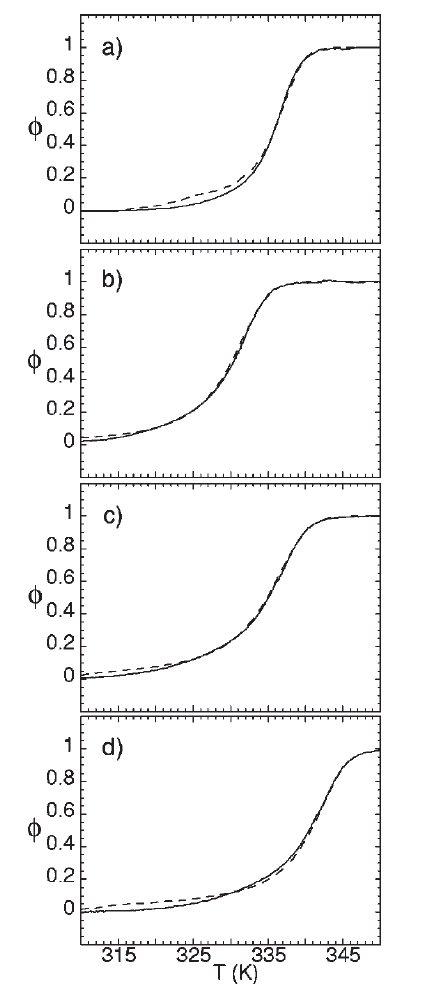
\includegraphics[scale=0.42]{Graphics/DNA/exp.png}
\caption{Experimental melting profiles (full lines) and theoretical results (dashed lines) for three different types of short heterogeneous DNA chains. The temperature is plotted against the average fraction of melted base pairs $\phi$. Subplots (a), (b) and (c) are the melting profiles for the three different DNA chains in a low concentration phosphate buffer solution. Subplot (d) uses the same DNA chain as in (c) but at a much higher concentrations \cite{Campa1998}.}
\label{fig:pbd_exp_test}
\end{figure}
%
Other studies which have investigated the thermodynamics of a heterogeneous PBD model have predicted a multi-step melting behaviour for some long DNA sequences agreeing with experimental observations \cite{Cule1997}. This has been investigated more recently in \cite{Theodorakopoulos2010}. 

The calculations of the eigenvectors and eigenvalues of the PB model go beyond the scope of this review, however. We have outlined the basic principles Peyrard et al. used to apply the transfer integral method. This method will be central to our axial shearing models for both DNA and collagen.

The FJC and WLC models describe the behaviour at a scale where complex polymers are coarse-grained to resemble a singular flexible strand. For DNA these models do not take into account the mesoscopic structure of the two backbones, and complementary base-pairs. As we are interested in DNA shearing and its effects on the base-pairs we will focus our attention on models that include some form of base-pair description. One such model proposed by de Gennes (2001) took a relatively simply approach in studying this behaviour which later became a foundation to other models that we will briefly review \cite{DeGennes2001,Chakrabarti2009,Prakash2011,Mishra2011a}. Collectively, these models showed excellent agreement with experiments when they were compared with results produced by Hatch et al (2008) \cite{Hatch2008}.

To model the force dependence of axial shear pulling de Gennes simplified the structure of DNA to a ladder ignoring the double helical twist, and approximated the backbone, and base-pair potentials to be harmonic with different stiffness constants $Q$ and $R$. By ignoring effects of finite temperature he described the Hamiltonian as a set of one-dimensional displacements for each strand distorted by a force $F$ with the extremities being pulled at either the 3'3' or 5'5' terminals of DNA \cite{DeGennes2001,Hatch2008}, namely
%
\begin{equation}
\label{deGennes_ham}
H=\sum_{-l/2}^{\infty}\frac{Q}{2}\left(u_{n+1}-u_{n}\right)^{2}+\sum_{-\infty}^{l/2}\frac{Q}{2}\left(v_{n+1}-v_{n}\right)^{2}+\sum_{-l/2}^{l/2}\frac{R}{2}\left(u_{n}-v_{n}\right)^{2}
\end{equation}
%
where $u_{n}$ and $v_{n}$ are the axial displacements for each strand with indices $n$ in the range of $-l/2 \leq n \leq l/2$. By defining a critical force for the breakage of a single base-pair to be $R|v_{n}-u_{n}|>f_{c}$ the equilibrium conditions derived from the Hamiltonian allow the overall rupture force $F_{c}$ to be expressed as \cite{DeGennes2001}:
%
%\begin{equation}
%\label{deGennes_eq}
%F_{c}=2 f_{c}\left[\varkappa^{-1}\tanh\left(\frac{\varkappa l}{2}\right)+1\right]
%\end{equation}
%
\begin{equation}
\label{deGennes_eq}
F_{c}=2 f_{c}\varkappa^{-1}\left(1-2\exp^{-\varkappa l}\right)
\end{equation}
%
%
where $\varkappa^{2}=2R/Q$, and $\varkappa^{-1}$ is defined as the number of base-pairs for which the tension is mainly on a single strand; a dimensionless quantity also known as the adjustment length. In this model most of the shear distortion is concentrated near the ends of the ladder structure resulting in larger base-pair axial displacements near $n=\pm l/2$. As we approach the centre of the structure the differential force across the base-pairs tend to zero \cite{DeGennes2001}.
%
\begin{figure}[t]
\centering
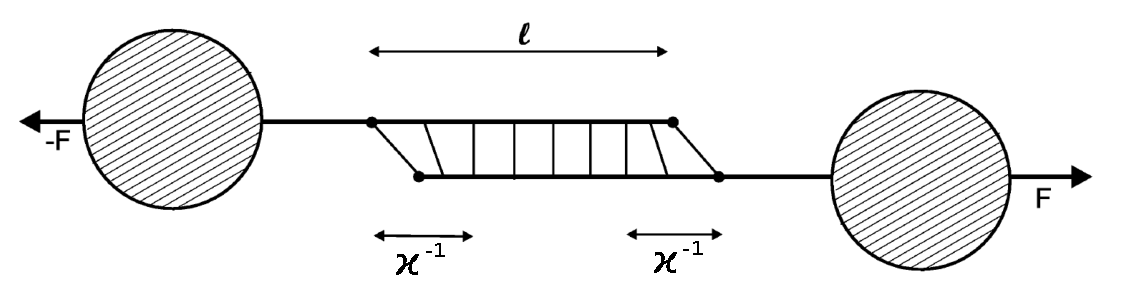
\includegraphics[scale=0.6]{Graphics/DNA/fig1_DeGennes2001.pdf}
\caption{A schematic diagram of the ladder model used by de Gennes. The equal and opposite forces distort the base-pairs over an adjustment length $\varkappa^{-1}$ at both ends of the ladder structure of length $l$. This figure was edited from \cite{DeGennes2001}.}
\label{fig:fig1_DeGennes2001}
\end{figure}
%
Experiments were able to test this model to a high degree of accuracy using magnetic tweezers to probe the shearing force of DNA \cite{Hatch2008}. There is an excellent agreement between experiment and the results predicted by \eqref{deGennes_ham} if we include the effects of a finite number of frayed ends in DNA. Results shown in \figref{fig1_Hatch2008} show that the best fit of de Gennes theory to experiment actually occurs when we assume 7 frayed base-pairs at each end of the ladder structure with $f_{c}=3.9$ pN, $\varkappa^{-1} = 6.8$ bp and stiffness constant ratio of $Q/R = 92.5$ \cite{Hatch2008}. 
%
\begin{figure}[h]
\centering
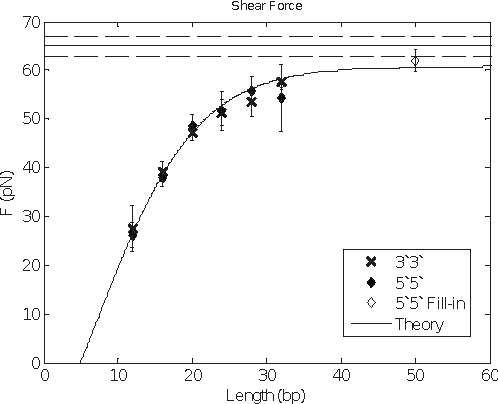
\includegraphics[scale=1]{Graphics/DNA/fig1_Hatch2008.pdf}
\caption{A match between the experimental results of pulling either 3'3' and 5'5' ends produced by Hatch et al with the best fit of \eqref{deGennes_eq}. The horizontal line at $65\pm3$ pN represents the forces characteristic of the over-stretching transitions as measured for the molecule. The upper and lower dashed lines correspond to 110\% and 90\% of the overstretched transition. This figure was taken from in \cite{Hatch2008}.}
\label{fig:fig1_Hatch2008}
\end{figure}
%
Matched by theory, the shear force as a function of number of base-pairs first increases linearly for short DNA lengths, and for larger lengths the critical force saturates below the asymptotic limit of entropic elasticity before the overstretched transition near $65$ pN. Both experiment and theory imply that the mechanical shear stress is localised at the ends of the molecule where the shear force is applied, and that the pulling techniques from 3'3' and 5'5' ends make no difference on the shearing force \cite{Hatch2008}. 

A generalisation of de Gennes model was later studied by Chakrbarti et al (2009) using a semi-microscopic vector model. Based on the same structure as shown in \figref{fig1_DeGennes2001} the model adds further detail to the Hamiltonian by including a stacking interaction term that is expressed as the interactions between nearest neighbours on the same strand, and the interactions between the nearest, and next nearest-neighbour nucleotides of the opposite strand. Keeping the backbone strands harmonic, and using a Lennard-Jones potential for the interaction along the complementary base-pairs the non-linear Hamiltonian can be expressed as \cite{Chakrabarti2009}:
%
\begin{align}
\label{chakrabarti_ham}
H=&\frac{Q}{2}\sum^{L}_{n=1}\left(|\vec{r}_{n+1}-\vec{r}_{n}|-a\right)^{2} +\left(|\vec{s}_{n+1}-\vec{s}_{n}|-a\right)^{2} + \\
&\sum^{L}_{n=1} V_{LJ}\left(|\vec{r}_{n}-\vec{s}_{n}|\right) + V'_{LJ}\left(|\vec{r}_{n+1}-\vec{s}_{n}|\right) + V'_{LJ}\left(|\vec{s}_{n+1}-\vec{r}_{n}|\right)\nonumber
\end{align}
%
where $\vec{r}_{n}$ and $\vec{s}_{n}$ are the position vectors of the $n$th nucleotide along the two backbone strands, $a$ is the equilibrium spacing between the bases along the backbone, and $L$ is the size of the overlap region shown in \figref{fig1_DeGennes2001}. The two additional potential terms labelled $V'_{LJ}$ represent the inter-strand stacking interactions that exist between the base-pairs of DNA. 
%
Though this vector model calculation takes a more complex approach to de Gennes, when coarse-grained, by solving and eliminating all displacements except those that couple directly to the force, \eqref{chakrabarti_ham} reduces to a general non-linear scalar model in terms of displacements projected along the chain. With the base-pair interaction still modelled by a Lennard-Jones potential the Hamiltonian becomes \cite{Chakrabarti2009}
%
\begin{align}
\label{chakrabarti_ham_1}
H=&\frac{Q}{2}\sum^{L}_{n=1}\left(u_{n+1}-u_{n}\right)^{2} +\frac{Q}{2}\sum^{L}_{n=1}\left(v_{n+1}-v_{n}\right)^{2} +\sum^{L}_{n=1}V_{LJ}\left(|u_{n}-v_{n}|\right)\\ &-Fu_{1}+Fv_{L}\nonumber
\end{align}
%
where $u_{n}$ and $v_{n}$ are now the displacements of the top and bottom parts of the ladder structure. Expanding the base-pair potential around the minimum and retaining terms up to the quadratic order we recover a harmonic approximation first studied by de Gennes where the force exceeds a critical value $F_{c} \sim f_{c}N$ for short chains, and $F_{c} \sim 2f_{c}\varkappa^{-1}$ for long chains \cite{Chakrabarti2009}. 

Extending this work further, the statistical mechanics of DNA shearing was later studied at a finite temperature using a Hamiltonian that was similar to the non-linear scalar displacement model of \eqref{chakrabarti_ham_1}. Calculating the shear force $F_{c}$ of DNA as a function of the number of base-pairs, this model developed by Prakash et al. (2011) found that an important factor in getting accurate results was dependent on the choice of values used for the adjustment length and single base-pair breakage force \cite{Prakash2011}. Keeping with the non-linear displacement model where the backbone strands are pulled along the molecular axis by an applied force $F$, the displacements of $i$th nucleotide from its equilibrium position are labelled by $u_{i}$, and $v_{i}$ leading to a Hamiltonian similar to \eqref{chakrabarti_ham}. Transforming the co-ordinate system the displacements of the Hamiltonian can be expressed as two independent components $H_{x}$, and $H_{y}$ in the constant force ensemble \cite{Prakash2011}.
%
\begin{equation}
H=H_{x}+H_{y}
\end{equation}
%
where
%
\begin{equation}
H_{x}=\sum^{N/2-1}_{i=-N/2}\frac{Q}{2}\left(x_{i+1}-x_{i}\right)^{2} - \frac{F}{\sqrt{2}}\left(x_{N/2}-x_{-N/2}\right)
\end{equation}
%
and
%
\begin{equation}
H_{y}=\sum^{N/2-1}_{i=-N/2}\frac{Q}{2}\left(y_{i+1}-y_{i}\right)^{2} + V\left(y_{i}\right) - \frac{F}{\sqrt{2}}\left(y_{N/2}-y_{-N/2}\right)
\end{equation}
%
The base-pair interactions in this model are represented by a potential that encompasses a hardcore repulsion to prevent the compression of base-pairs with respect to its equilibrium, as well as long range interactions. The potential is expressed as
%
\begin{equation}
\label{pe_shikha}
V\left(y_{i}\right)=-\frac{\epsilon}{\left(1+\frac{2y^{2}_{i}}{\sigma^{2}}\right)^{3}}
\end{equation}
% 
where $\epsilon$ is the depth of the potential, and $\sigma$ is the diameter of DNA. In calculating the average positions, $H_{x}$ simplifies $\langle x_{n}\rangle$ to an integral of a Gaussian that can be solved analytically to give 
%
\begin{equation}
\langle x_{n}\rangle = \frac{F}{\sqrt{2}\kappa}n
\end{equation}
%
which agrees with the result found by de Gennes \cite{Prakash2011,DeGennes2001}. The potential term $V\left(y_{i}\right)$ gives the partition function integral of $H_{y}$ a non-Gaussian form and therefore needs to be calculated numerically. Calculating the average displacement quantities Prakash et al. was able to study how the DNA shearing was distributed along the molecule as well as the energies associated with backbone and base-pair stretching. In this constant force model, the shear force needed to separate two strands of DNA was calculated by defining a critical distance $\bar{y}$ needed to rupture a single base-pair. By differentiating the potential \eqref{pe_shikha} with respect to $y$, the critical force for a single base-pair was fitted to be close to the values used by Hatch et al. to fit their experimental data of $f_{c}=4.1$ pN if $y = 2.38$ \AA. The expression for the critical force as derived by Prakash et al. was found to be \cite{Prakash2011}:
%
\begin{equation}
F_{c}=\sqrt{2}\kappa\left(\langle y_{N/2}\rangle - \langle y_{\left(N/2-1\right)}\rangle\right) + 2f_{c}
\end{equation} 
%
When the base-pairs at the ends of that ladder structure $\langle y_{N/2}\rangle$ reach an axial displacement of $\bar{y}$, the point of shearing, the values of $\langle y\rangle$ can be determined. Prakash's results for molecules with 10-60 base-pairs are shown as the dotted curve plotted in \figref{fig6_Prakash2011} and compare well with the experimental results of Hatch et al. 

Alternatively, for a constant extension method the average force is calculated from the amount of work needed to keep the extension of the ladder a distance $y$. From the Hamiltonian the work done by the base-pairs was calculated using the partition function with the constrained displacements imposed using two delta functions for each end, $\delta\left(y_{-N/2}-y\right)\delta\left(y_{N/2}-y\right)$, Prakash et al. described the work done as a function of $y$ by the relations \cite{Prakash2011}:
%
\begin{equation}
\label{shikha_workdone}
W\left(y\right) = \frac{1}{\beta}\left[\ln Z_{N+1}\left(y\right)-\ln Z_{N+1}\right]
\end{equation}
%
where
%
\begin{equation}
Z_{N+1}\left(y\right)=\int \prod^{N/2}_{i=-N/2}dy_{i}\delta\left(y_{-N/2}-y\right)\delta\left(y_{N/2}-y\right)\exp\left(-\beta H_{y}\right)
\end{equation}
%
and 
%
\begin{equation}
Z_{N+1}\left(y\right)=\int \prod^{N/2}_{i=-N/2}dy_{i}\exp\left(-\beta H_{y}\right)
\end{equation}
%
The critical force, $F_{c}$, is now simply the first derivative of \eqref{shikha_workdone} with respect to $y$ taking a value that represents the separation length needed to break a single base-pair $y_{c}$. The dashed curve shown in \figref{fig6_Prakash2011} is plot using the constant extension ensemble with $y$ having a value of $2.0$ \AA. 

Even though both these methods produce slightly different results for molecules of small lengths which later converge for molecules of larger $N$, both these methods agree well with results found by Hatch \cite{Prakash2011}. 
%
\begin{figure}[H]
\centering
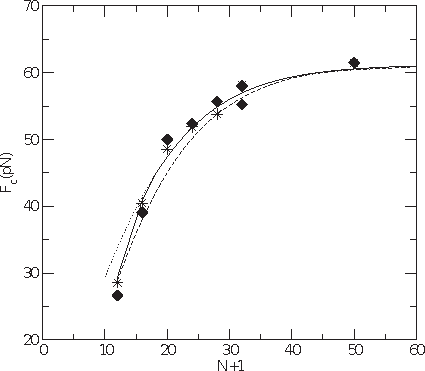
\includegraphics[scale=1.5]{Graphics/DNA/fig6_Prakash2011.pdf}
\caption{Results from the constant force method are shown by the dotted curve, and the constant force method is shown by the dashed curve of the critical force $F_{c}$ as a function of the base-pairs. The experimental results of Hatch et al are shown by diamonds for 5'5' pulling, and stars for 3'3' pulling. This figure was taken from \cite{Prakash2011}.}
\label{fig:fig6_Prakash2011}
\end{figure}
%
Compared with experimental data \cite{Prakash2011,Hatch2008} these models agree well with axial shearing of DNA \figref{fig6_Prakash2011}. For long molecular lengths the models reach an important asymptotic limit giving reasonable fitting parameters to the shearing force of a single base-pair, and stiffness constant ratio between the the backbone and base-pair. These models do not take into account breakage of base-pairs.

\newpage
\section{Collagen}

Collagen is a naturally occurring protein that is a central structural component of multicellular organisms most abundantly found in animals. Forming the major component of the extracellular matrix and connective tissue collagen exist in several distinct types discussed extensively in \cite{Shoulders2009,Fratzl2008,Berg2010,Brinckmann2005}. The collagen subtypes can be found in tissues such as skin, tendon, bone, and cartilage with 80 to 90 percent of the collagen in the human body consisting of types I, II, and III. These collagen molecules pack together to form elongated fibrils of similar structure.  

Reinforcing biological tissues, collagen molecules also pack together to create fibrous polymers that are the major building blocks of all types of load-bearing tissues making the mechanical properties of collagen extremely important \cite{Buehler2006}. In bone and dentin, collagen is combined with mineral to yield very stiff tissues that transmit the force from muscles to bones enabling mammals to physiologically move. In tendon or the cornea, collagen is combined with other organic molecules, such as proteoglycans for different biological functions \cite{Fratzl2008,Bozec2005a,Bozec2007,Ottani2001}.

Due to the limitations in performing mechanical testing on the nanometre and micrometre scale only very recent studies have been initiated to measure the mechanical properties of substructures like collagen fibrils, and tropocollagen \cite{Bozec2005a,Bozec2007,Buehler2006a}.

\subsection{Collagen Structure}

Similar to DNA as well as other proteins, the collagen molecule has a hierarchical structure arising from the interactions of amino acid molecular groups at different levels. Three parallel polypeptide chains, also known as $\alpha$-chains, are made up of repeating amino acid triplets that intertwine in an overall right-handed coil to form the secondary structure of the collagen molecule which is approximately 300 nm long and 1.5 nm wide. This structure is known as a triple helix \cite{Shoulders2009,Fratzl2008,Berg2010,Brinckmann2005,Ramachandran1954,Ottani2001,Bozec2005a,Bozec2007,Buehler2006a}.

\begin{figure}
\centering
\subfloat[]{\label{fig:polypeptide}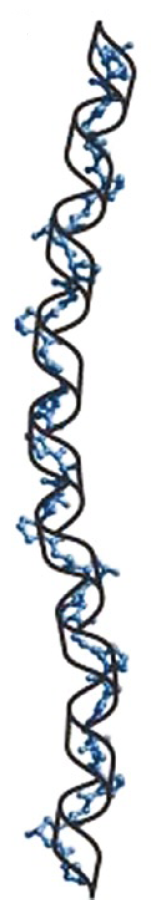
\includegraphics[width=0.08\textwidth]{Graphics/Collagen/polypeptide.png}}
\hspace{20 mm}                
\subfloat[]{\label{fig:polypeptide_sapcefilling}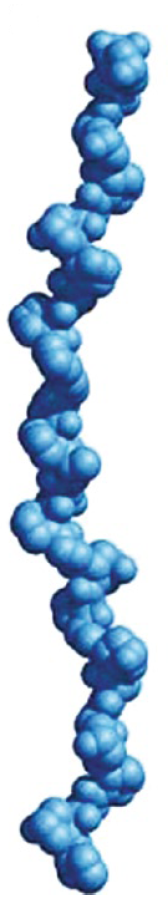
\includegraphics[width=0.09\textwidth]{Graphics/Collagen/polypeptide_spacefilling.png}}
\hspace{20 mm}
\subfloat[]{\label{fig:collagen_molecule}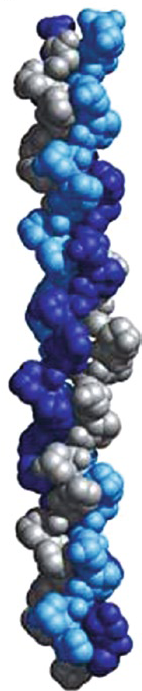
\includegraphics[width=0.1\textwidth]{Graphics/Collagen/tropocollagen.png}}
\caption{Formation of the collagen triple helix from three polypeptide chains. Each polypeptide has a left-handed helical structure as shown in \figref{polypeptide}. A space-filling diagram of the same polypeptide is shown in \figref{polypeptide_sapcefilling}. \figref{collagen_molecule} illustrates three polypeptide chains wrapping around one another with a right-handed twist. (Figure 4.12a, b and c taken from \cite{Nelson2004})}  
\label{fig:polypeptide_to_tropocollagen}
\end{figure}

The amino acids are bound together by peptide bonds which are strong covalent bonds between the carboxyl group and the amino group of each amino acid. Each of the three polypeptides in collagen contains 1000 amino acid residues forming a primary structure that is coiled into a left-handed non-$\alpha$ extended helix. The helix is caused by a steric repulsion of the five-membered heterocycle Pro rings in the hydroxyproline and the proline residues \cite{Shoulders2009,Bhattacharjee2005}. 

\begin{figure}[htp]
\centering 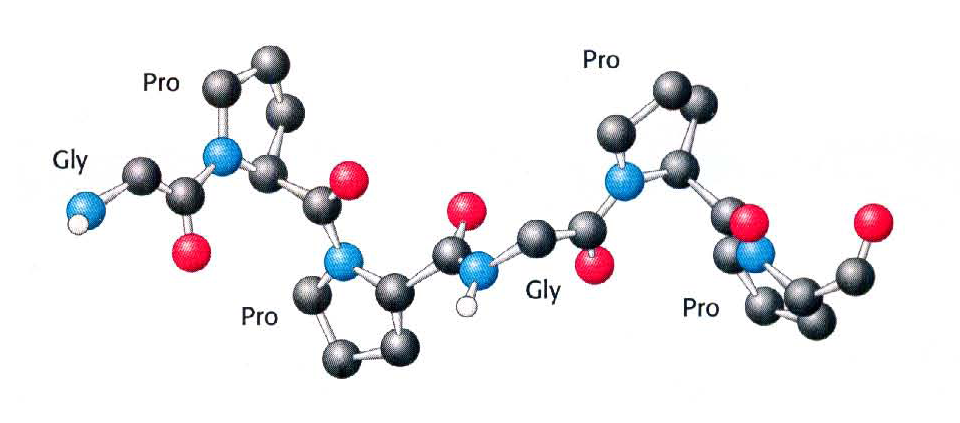
\includegraphics[scale=0.3]{Graphics/Collagen/polypeptide_section_freeman.png}
\caption{A section of a polypeptide showing two amino acid triplets of GlyProHyp covalently bonded by a peptide bond. It also shows the steric repulsion of the heterocyclic rings. (From Fig. 2-39 in \cite{Berg2010})}
\label{fig:col_polyp_sec}
\end{figure}

The tight molecular packing of the three polypeptide chains results in a glycine residue being close to the central core of the triple helix \cite{Shoulders2009,Bhattacharjee2005,Berg2010}. The amino acids in the Xaa and Yaa positions of collagen are often proline and hydroxyproline residues respectively. The compact space near the centre of the triple helix is unable to accommodate any of the larger groups of any amino acid and therefore to maintain stability the large Pro rings are positioned on the outermost part of the triple helix.
  
\begin{figure}
\centering
\subfloat[]{\label{fig:old_td_collagen}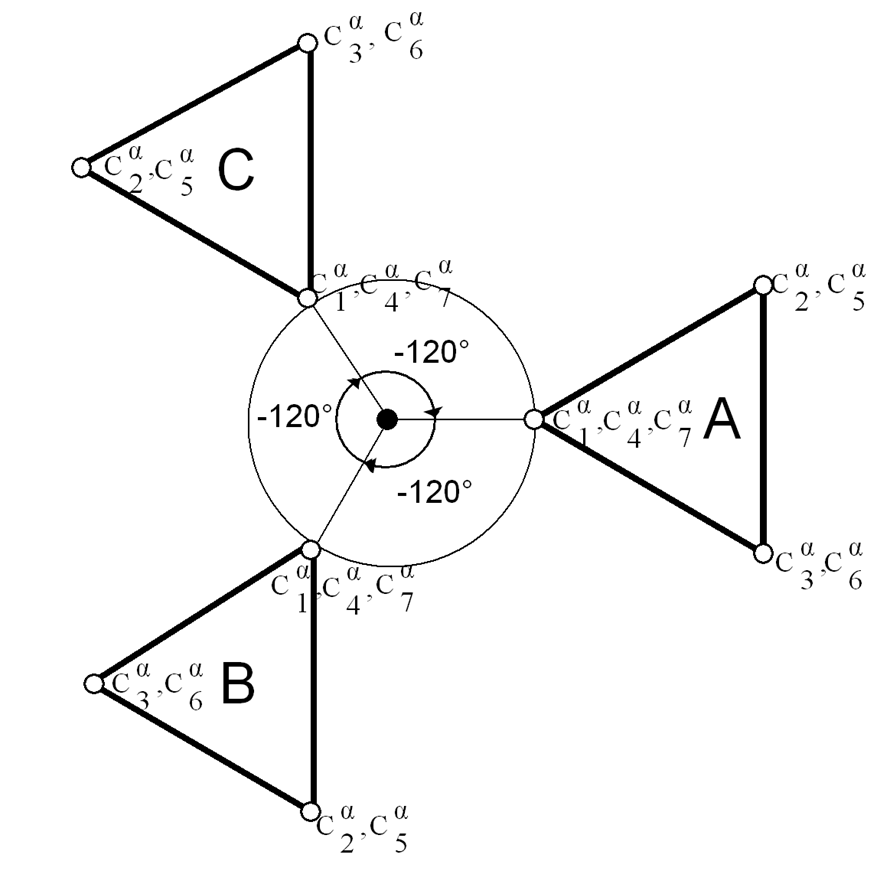
\includegraphics[width=0.275\textwidth]{Graphics/Collagen/old_td.png}}                
\subfloat[]{\label{fig:new_td_collagen}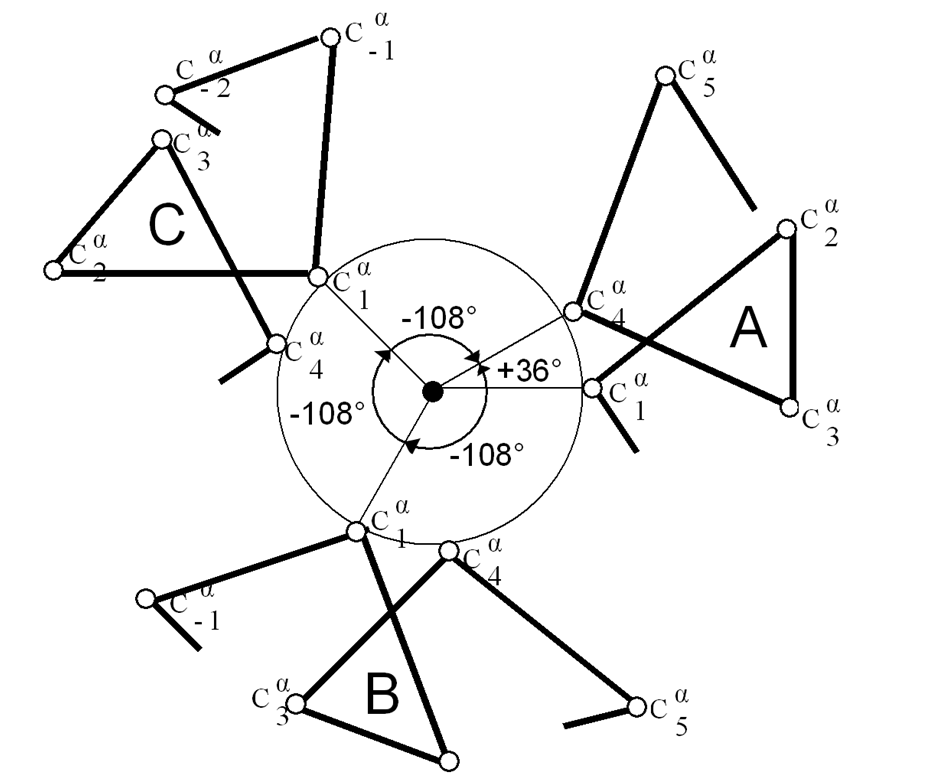
\includegraphics[width=0.3\textwidth]{Graphics/Collagen/new_td.png}}
\subfloat[]{\label{fig:td_freeman}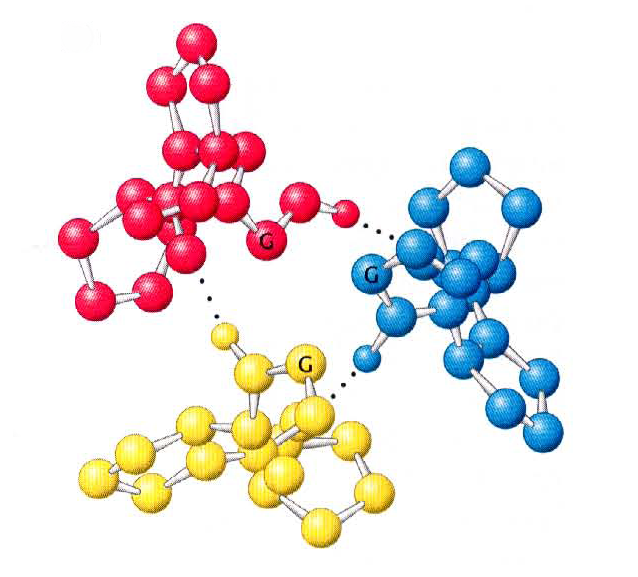
\includegraphics[width=0.3\textwidth]{Graphics/Collagen/td_collagen_freeman.png}}
\caption{A top-down view of the collagen triple helix. The far left \figref{old_td_collagen} was the original structure proposed by Ramachandra \cite{Ramachandran1954} (Figure 1a from \cite{Bhattacharjee2005}). This was later refined by Ramachandra, proposing a coiled structure \cite{Ramachandran1955} in \figref{new_td_collagen} (Figure 1b from \cite{Bhattacharjee2005}). \figref{td_freeman} is a molecular top-down illustration of coiled coil triple helix. } 
\label{fig:top_down_view}
\end{figure}

Ramachandra and Kartha first proposed the first prototype of the right-handed triple helix structure for the collagen molecule in 1954 using X-ray diffraction pictures from different sources \cite{Ramachandran1954}. Their initial structure comprised of three staggered left-handed polypeptides related by a three fold screw symmetry about a common axis, with approximately three residues per turn (\figref{old_td_collagen}) \cite{Ramachandran1954,Bhattacharjee2005}. All peptide bonds were positioned in a trans position and had two hydrogen bonds within each triplet stabilising the triple helix \cite{Ramachandran1954}. This model was later updated to fit observations from X-ray diffraction of stretched collagen fibres which proposed a coiled coil triple helical structure indicating approximately 3.33 residues per turn of the left handed minor helix of each chain \figref{new_td_collagen} \cite{Ramachandran1955}. The major right handed helix had 30 residues per turn. The neighbouring helices in the triple helical assembly are thus related by a twist of $-108^{\circ}$ and rise of $\sim 2.86$\AA \cite{Ramachandran1955,Bhattacharjee2005}. However, this model still caused problems until a refinement by Rich \& Crick showed only one inter-strand hydrogen bond existed per amino acid triplet \figref{schematic_3strand_section} \cite{Rich1955}. 

The collagen triple helix is stabilised by inter-chain hydrogen bond networks. Within each amino acid triplet, one hydrogen bond forms between the amide hydrogen (NH) atom of glycine, a hydrogen bond donor, in one chain and the carbonyl oxygen (C=O) atom of residue X in an adjacent strand, a hydrogen bond acceptor \cite{Ramachandran1954,Rich1955} \figref{schematic_3strand_section}.  Additional stability comes from other weak hydrogen bond systems where the hydrogen of a residue is weakly bonded to the carbonyl oxygen atom of another residue in an adjacent strand, and the two hydrogen atoms of glycine are weakly bonded to the carbonyl oxygen atom of another glycine located in one of the adjacent strands \cite{Perczel2009}.

\begin{figure}[htb]
\centering
\subfloat[]{\label{fig:schematic_3strand_section}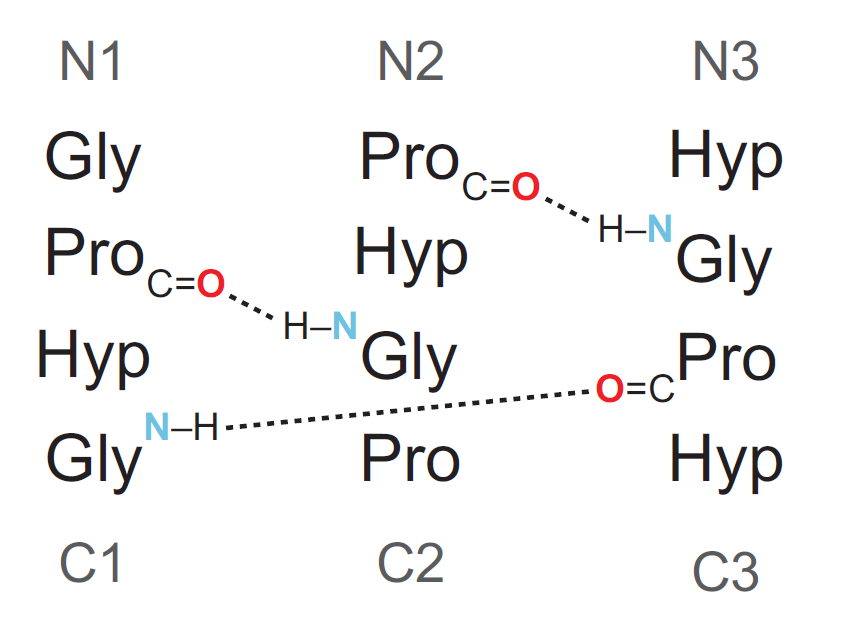
\includegraphics[width=0.3\textwidth]{Graphics/Collagen/shoulders_schematic_polypeptide_3strand.png}}    
\hspace{20mm}            
\subfloat[]{\label{fig:3strand_section}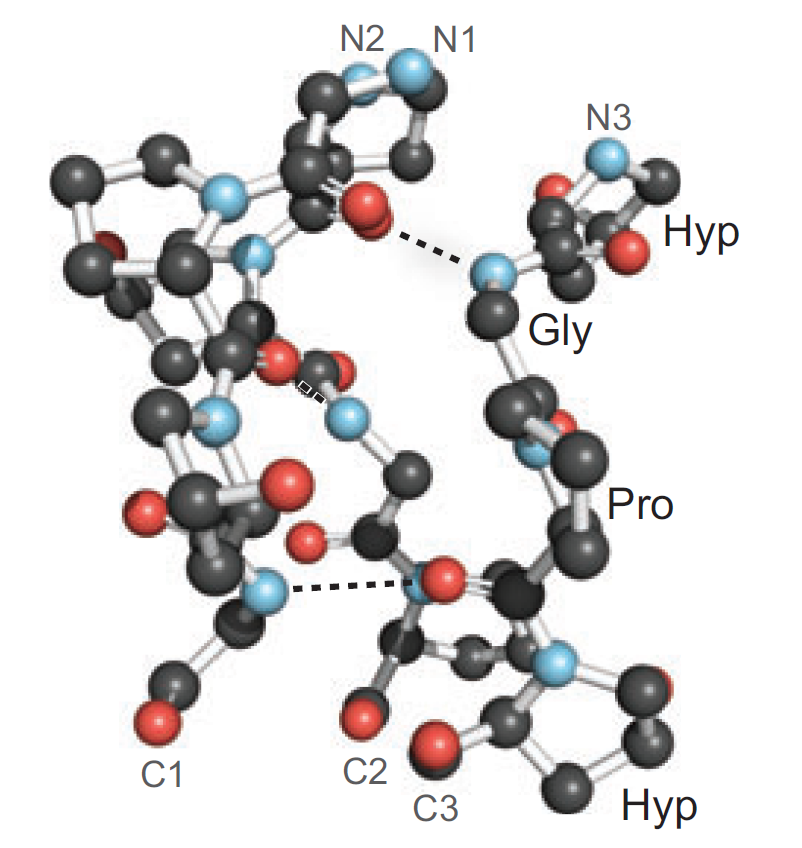
\includegraphics[width=0.3\textwidth]{Graphics/Collagen/shoulders_polypeptide_3strand.png}}
\caption{An illustration showing a segment of the collagen triple helix. A schematic diagram of the segment shows the hydrogen bonds between the amino acid triplet in each polypeptide \figref{schematic_3strand_section} and the ball and stick image shown in \figref{3strand_section} shows a 3D representation of the strong hydrogen bonds, and three polypeptides \cite{Shoulders2009}. (Figures 1c and 1d from \cite{Shoulders2009}.)} 
\label{fig:collagen_segment}
\end{figure}

%\begin{figure}[htp]
%\centering 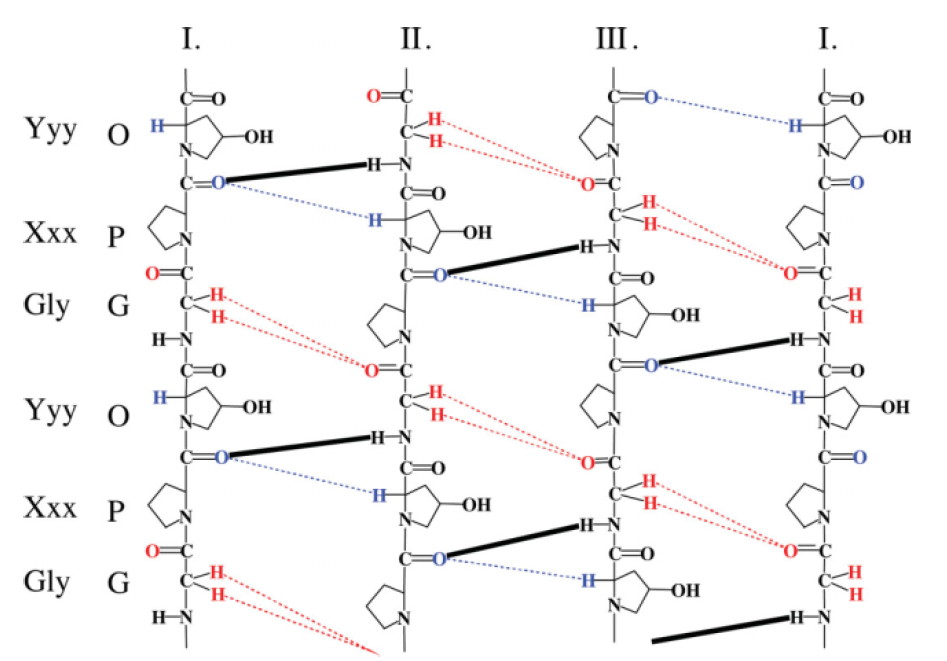
\includegraphics[scale=0.3]{Graphics/Collagen/perczel_collagen_h_network.png}
%\caption{An illustration showing the hydrogen bond networks in tropocollagen. The strong hydrogen bonds are drawn in a strong black lines and the weak hydrogen bonds are depicted by the dashed red and blue lines. The first strand, I, is duplicated at the right to better picture the circular nature of the tropocollagen and its H-bond network \cite{Perczel2009}. (Figure 1 from from \cite{Perczel2009}.)}
%\label{fig:detailed_collagen_h_network}
%\end{figure}

%\begin{figure}[htp]
%\centering 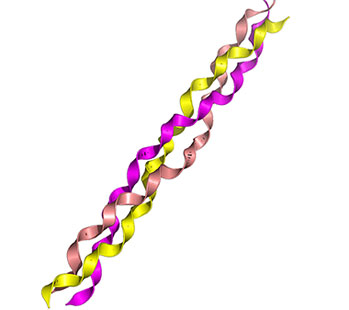
\includegraphics[scale=0.6]{Graphics/Collagen/Collagen1.jpg}
%\caption{}
%\label{fig:col1}
%\end{figure}

%\begin{figure}[htp]
%\centering 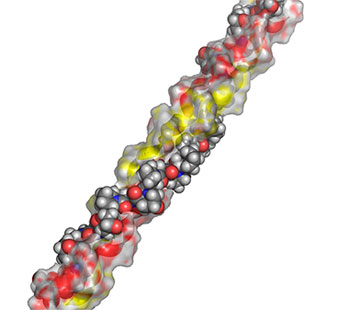
\includegraphics[scale=0.6]{Graphics/Collagen/Collagen2.jpg}
%\caption{}
%\label{fig:col2}
%\end{figure}


\subsection{Collagen Mechanics}

Extensive studies of the mechanical properties of collagen molecules have been made. In single molecule pulling experiments different set-ups have shown that the force-extension behaviour in the entropic elasticity region can be modelled accurately by using the WLC model. At larger forces the increase in tensile strain causes the mechanical behaviour of the molecule to move into the energetic elasticity region where the WLC model fails. We expect to observe the stretching and breaking of hydrogen bonds followed by the deformation of covalent bonds \cite{Buehler2007}. Results from some of the early experiments probing the entropic response of collagen molecules are shown as force-extension curves in \figref{tc_entropic_response}. Investigations by Sun et al. used optical tweezers to stretch human procollagen molecules of type I and II, the precursor form of collagen monomers. The chemical attachment to the beads was achieved by using the abundant amount of disulfide bonds present at the terminal ends of the procollagen molecules. Biotinyated type II procollagen was purified through a desalted column and coated on streptavidin-coated polystyrene beads; one terminal was fixed to a stationary bead on a moving plane while the other terminal was attached to a free bead trapped by optical tweezers \cite{Sun2004}. The molecule was stretched by moving the plane of the fixed bead and measuring the elastic response of the trapped bead using an optical laser \cite{Sun2001}. Fitting their data to the WLC model they found that the collagen monomer had a persistence length of $L_{p} \sim 15 \text{ nm}$ and a contour length of $L \sim 300 \text{ nm}$ \cite{Sun2001,Sun2004}.

\begin{figure}[H]
\centering
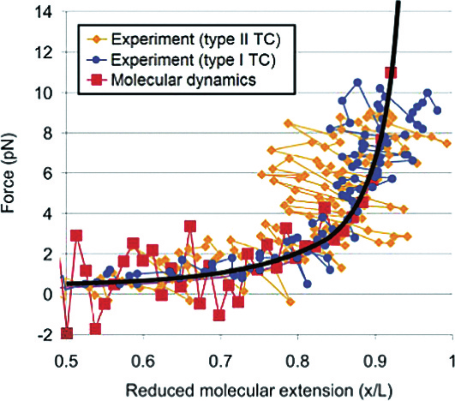
\includegraphics[scale=1]{Graphics/Collagen/Fratzl_2008_fig8p22.pdf}
\caption{A plot of molecular extension of a single collagen molecule in the entropic regime (F \textless 14 pN). The experimental results on type I and type II collagen molecules were reported in \cite{Sun2002,Sun2004} and the MD results were obtained from a study by Buehler et al. using a mesoscale model to predict the force-extension response of a collagen molecule \cite{Buehler2007}. Image was taken from \cite{Fratzl2008}.} 
\label{fig:tc_entropic_response}
\end{figure}

In AFM experiments by Bozec et al. insoluble tropocollagen molecules with cleaved terminals were pulled from a surface without a covalent coupling between the tip and the molecule. This method had no control over the binding processes resulting in cases where multiple molecules were being pulled off the surface, and variations in position where the probe becomes bound to the molecule along its length. Repeat experiments were used to differentiate between single and multiple stretching events. The mechanical properties obtained from this  method of stretching collagen molecules was determined to be only representative of the actual length of the monomer stretched rather than the entire molecule \cite{Bozec2005a}. Shown in \figref{bozec_tc_entropic_response} are the results from these measurements fitted to the WLC model for small extensions. Similar experiments on rat tail tendon by Gutsmann et al. found that the steep increase in force was a result of stretching individual collagen molecules. Their force-extension curves were similar to the ones found by Bozec et al. \cite{Bozec2005a,Gutsmann2004}. They determined the effective contour length of the pulled collagen monomer by fitting their data to the WLC model using a persistence length of $L_{p} \sim 0.4 \text{nm}$.  

Observations made by Bozec et al. did suggest that a proportion of the force-extension curves obtained did feature a discontinuity, thought to be the result of structural changes within the sample, exhibiting a transition to different mechanical behaviour. In data sets where peaks did not exhibit a discontinuity it was found that the WLC model failed at larger extensions \cite{Bozec2005a}. 

\begin{figure}[H]
\centering
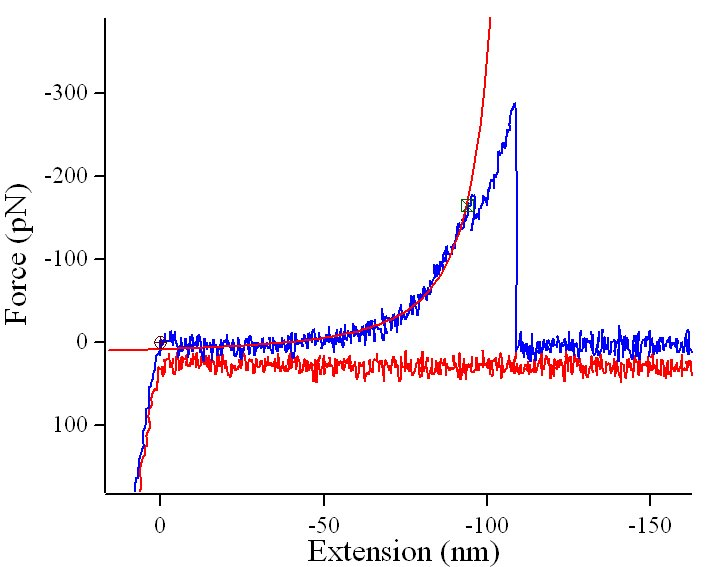
\includegraphics[scale=0.25]{Graphics/Collagen/Bozec_2005.jpg}
\caption{A force extension curve from pulling collagen molecules from a surface using atomic force microscopy. A persistence length of $L_{p} \sim 0.4 \text{ nm}$ was used to fit the WLC model to the data. The discontinuity found in this plot at an extension of approximately 100 nm occurred in 20\% of cases across an entire data set.} 
\label{fig:bozec_tc_entropic_response}
\end{figure}

Recently, molecular dynamic simulations have been used get a better understanding of the nanomechanical properties of tropocollagen molecules \cite{Buehler2007, Lorenzo2005, Buehler2006a, Gautieri2010}. In the full atomistic model calculations by Buehler et al. simulations were run using two types of force field parameters to include the atomistic interactions in proteins: a non-reactive CHARMM force field which provides harmonic and anharmonic terms to describe covalent, van der Waals, and electrostatic interactions, and a reactive ReaxFF force field which includes the dissociation of chemical bonds under deformation \cite{Buehler2006a, Buehler2007}. Fixing one end of the tropocollagen molecule by applying constraints to each of the three carbon atoms, a mechanical load is applied axially using steered molecular dynamics to obtain a force-extension relationship. In these types of MD simulations an external force is applied through a virtual spring with a known stiffness constant to steer the tropocollagen molecule along a path to simulate mechanical stretching also known as steered molecular dynamics (SMD). In both cases Buehler et al. found the results to agree well with experiment for small strains up to 10\% strain but deviated strongly at large strains. The maximum tensile force in the collagen molecule reached , $F \sim 2.35 \times 10^{4} \text{ pN}$ \figref{buehler_cg_model_results}. At $T=300K$ the persistence length was found to be $L_{p} \sim 23.4 \text{ nm}$. Running a simulation for pulling a single polypeptide out of the tropocollagen molecule he found the strength to be $\sim 0.713 \times 10^{4} \text{ pN}$ reaching 3.7\% tensile strain \cite{Buehler2006a}.

\begin{figure}[H]
\centering
\subfloat[]{\label{fig:buehler_cg_model_results}\centering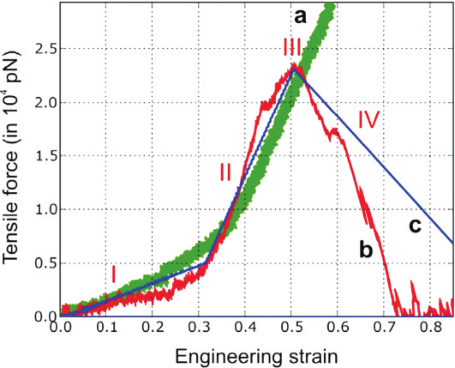
\includegraphics[scale=0.7]{Graphics/Collagen/Fratzl_2008_fig8p2.pdf}}
\hspace{5mm}
\subfloat[]{\label{fig:buehler_cg_model}\centering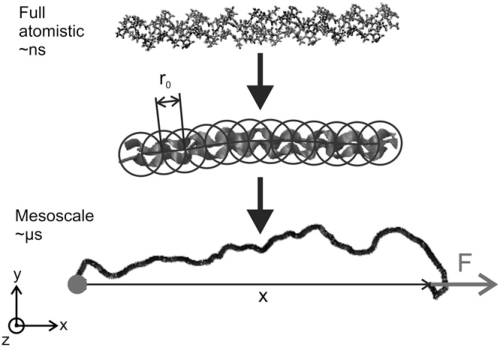
\includegraphics[scale=0.7]{Graphics/Collagen/Buehler_2007_fig4.pdf}}
\caption{The force extension behaviour from the atomistic simulations of a single collagen molecule with $L \sim 8.4\text{ nm}$ are plotted in \figref{buehler_cg_model_results}.  The methods used in these MD simulations had a non-reactive CHARMM force field (a), a reactive ReaxFF force field (b), and a reactive mesoscale model (c) shown in \figref{buehler_cg_model}. The tensile deformation of the molecule starts with the uncoiling of the triple helical structure (I), at larger strains the modulus gradient increases to reflect the stretching of covalent bonds (II). In phase (III) the molecule breaks with a rapid decay of force in phase IV \cite{Buehler2006a, Buehler2007}.} 
\label{fig:buehler_model}
\end{figure}

Taking a coarse-grained approach in the mesoscopic model, Buehler et al. simplified the tropocollagen molecule to a collection of beads. At this level information about the biochemical features within the molecule is lost \figref{buehler_cg_model}. Each bead represents approximately 10 protein atoms having a radius of 7 \AA. Again, one end of the molecule in the simulation is fixed while a force is applied to the other, thus extending the molecule. The MD results shown in \figref{tc_entropic_response} demonstrate a very good agreement with experimental results in the entropic regime. A fit to the WLC model found the persistence length to be $L_{p} \sim 16 \text{ nm}$ where the contour length of the molecule was $L = 301 \text{ nm}$ \cite{Buehler2007}.

In a separate MD study, Gautieri et al. used a coarse-grained MARTINI force-field to model the collagen molecule after making modifications to include parameters that described a hydroxyproline amino acid residue and incorporated the triple helical conformational structure of collagen. All the amino acids are modelled by mapping four non-hydrogen atoms into one bead, and the number of beads used to model a specific residue is decided from the dimensions of the side chain of the amino acid. In determining the force field parameters that describe the triple helix structure of collagen, bond lengths between backbone beads, bonding angles, and dihedral angles were analysed using five collagen-like molecules. These parameters were then used in SMD simulations to obtain a reference force-extension behaviour to determine the elastic stiffness for the potential energy terms in bond stretching, angle deformation, and dihedral deformations \cite{Gautieri2010}. 

\begin{figure}[H]
\centering
\subfloat[]{\label{fig:gautieri_cg_model_comp}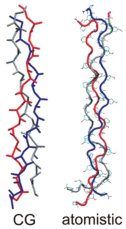
\includegraphics[scale=1.2]{Graphics/Collagen/Gautieri_2010_fig3b.pdf}}
\hspace{10mm}
\subfloat[]{\label{fig:gautieri_cg_model}\raisebox{0.2\height}{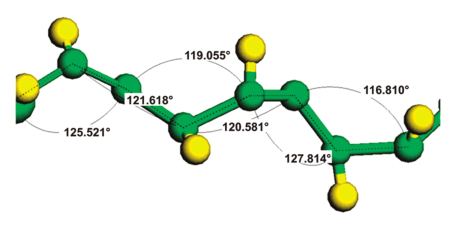
\includegraphics[scale=0.8]{Graphics/Collagen/Gautieri_2010_fig1.pdf}}}
\caption{A comparison between the full atomistic and coarse-grained structures of collagen. Image \figref{gautieri_cg_model} is a detailed view of the coarse grained polypeptides in collagen showing the angles between the backbone beads. The bond lengths between backbone beads, bonding angles, and dihedral angles were computed on the basis of five different collagen molecules. Gautieri et al. obtained a bond reference length $d_{b} = 0.365 \pm 0.07$ nm, a bonding reference angle $\varphi_{a} = 119.2 \pm 8.72^{\circ}$, and a dihedral reference angle $\Psi_{d} =-89.3 \pm 9.76^{\circ}$ \cite{Gautieri2010}.} 
\label{fig:gautieri_MARTINI_model}
\end{figure}

Focusing our attention on the backbone, the spring constant $K_{b}$ was calculated by simulating a single glycine-proline structure and then matching a best fit of the force-extension curve to the full atomistic simulations computed using GROMACS with GROMOS96 43a1 force field parameters. Shown in \figref{gautieri_backbone}, a best fit was found for $K_{b} = 1250 \text{ kJ mol}^{-1} \text{ nm}^{-2}$. Further details of the Extended MARTINI force fields are described comprehensively in \cite{Gautieri2010, Marrink2007, Monticelli2008}. The simulation of a $8 \text{ nm}$ collagen molecule using the coarse-grained model had a stiffness of $1052 \pm 51.23 \text{ pN nm}^{-1}$  up to 15\% strain as shown in \figref{gautieri_results}. In simulating a 300 nm human type I collagen molecule Gautieri et al. obtained a persistence length of $L_{p}=51.5 \pm 6.7 \text{ nm}$.

\begin{figure}[H]
\centering
\centering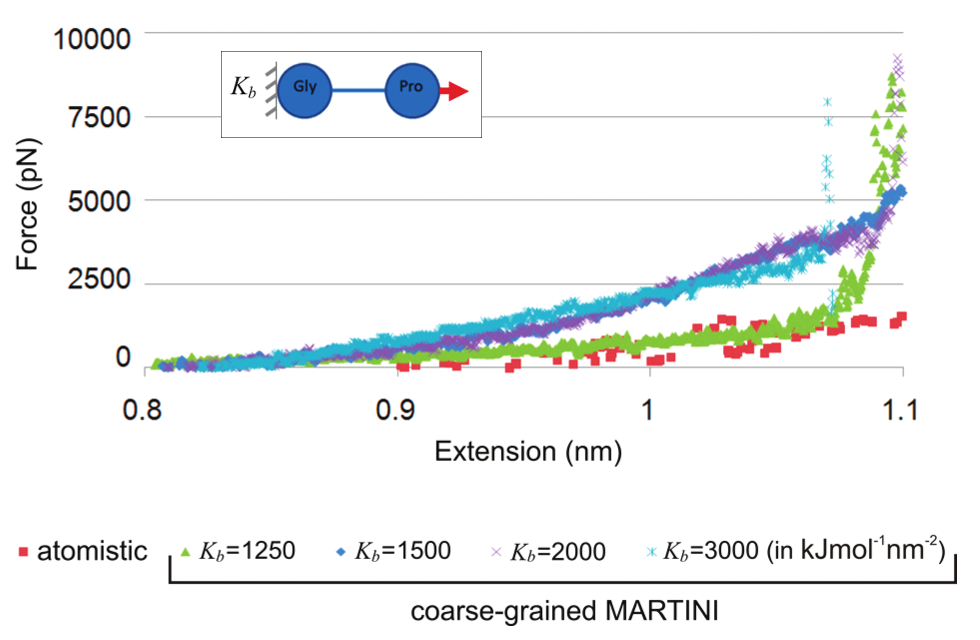
\includegraphics[scale=0.3]{Graphics/Collagen/Gautieri_2010_fig2_combined.png}
\caption{A plot determining the elastic stiffness of the backbone spring constant. The inset diagram is an illustration of the MD simulation studied with the results plotted for various values of $K_{b}$. Data comparison with the atomistic calculations suggest $K_{b} = 1250 \text{ kJ mol}^{-1} \text{ nm}^{-2}$ \cite{Gautieri2010}.} 
\label{fig:gautieri_backbone}
\end{figure}

\begin{figure}[H]
\centering
\label{fig:}\centering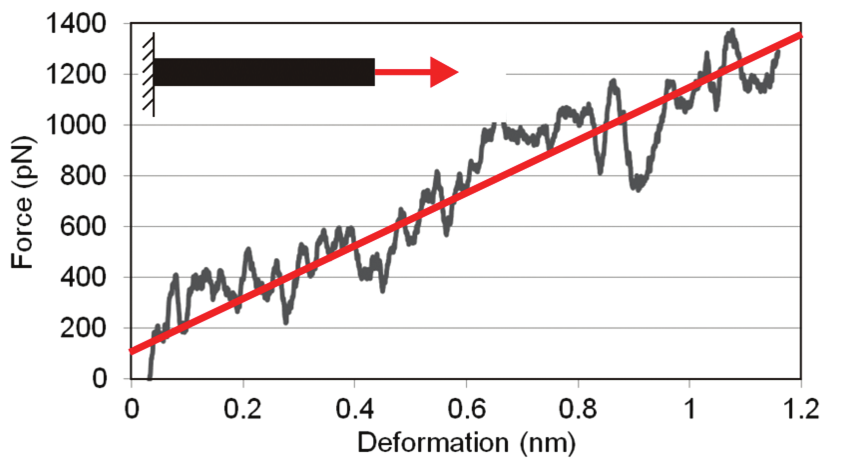
\includegraphics[scale=0.3]{Graphics/Collagen/Gautieri_2010_fig4a.png}
\caption{Force-extension plot of a $8 \text{ nm}$ collagen molecule using the Extended MARTINI force field up to 15\% strain (1.2 nm).} 
\label{fig:gautieri_results}
\end{figure}

Apart from a few pulling experiments of collagen molecules, most of the work described has been focused on the work done by MD simulations giving valuable information on the collagen backbone stiffness. Unfortunately no experimental investigations on the axial shearing of collagen molecules have been found.
